\section{Detecting Collusion: Market Evidence and Tests for Bid Rigging}\label{sec:13-detection}

An outsider who suspects collusion usually sees prices, quantities or bids, and little else. This section asks
what such evidence can reveal. \Cref{sec:13-market-evidence} reviews the kinds of evidence on which a finding of
collusion can rest. They are pricing patterns, measures of price elevation, facilitating practices, structural
conditions, internal records, and the plus factors of cartels and bidding rings. The remaining subsections develop
formal tests for public procurement.

Public procurement is among the settings in which collusion is most often prosecuted, and statistical detection
methods are most developed there. A buyer, such as a highway department or a school district, solicits sealed bids for a
contract and awards it to the lowest bidder. In procurement, bid rigging (\cref{sec:13-intro}) takes the form of an
agreement among bidders about who will win a contract and at what price. \citet[p.~1]{PorterZona1993} show how common it is. Between 1982 and 1988,
bid rigging or price fixing in auction markets accounted for more than half of the criminal antitrust cases filed
by the U.S.\ Department of Justice. In school milk alone, \citet[p.~1]{PorterZona1999} count investigations in more than twenty
states and guilty pleas in at least a dozen. They also report fines above \$90 million and about ninety people sent
to jail.

The buyer observes the bids and the identities of the bidders. It does not observe their costs. A ring that knows
this can choose bids that look competitive. Detection therefore follows the strategy of the rest of this chapter.
We write down a model of noncooperative bidding, derive restrictions on observable bids, and ask whether a group
of suspected firms violates restrictions that other firms satisfy. A rejection shows that the suspected group
behaves differently. It does not by itself prove an agreement, because the model may be misspecified for that
group alone. \Cref{sec:13-detection-theory} develops the theory of such tests. \Cref{sec:13-pz93,sec:13-pz99}
apply it to highway paving on Long Island and to school milk in Ohio. Detection based on the comparison of auction
formats, as in the test for mill collusion of \citet{AtheyLevinSeira2011}, is treated in \cref{ch:auction-empirics}.
Page and table references to the two papers of Porter and Zona are to their NBER working-paper versions, and ``WP
p.'' denotes a working-paper page.

\subsection{Market evidence, plus factors and screens}\label{sec:13-market-evidence}

Detection is the central challenge in the control of coordinated price elevation \citep[p.~256]{Kaplow2013}. Firms
hide conduct that may be illegal, and an aggressive search for it produces false positives that chill competitive
behavior. This subsection asks what an outsider can infer from market evidence before we turn to the specialized
tests for procurement. It draws on two book-length treatments. \citet[chs.~10--11]{Kaplow2013} classifies the
evidence on which a finding of coordination can rest. \citet[chs.~11--12]{MarshallMarx2012} catalog the
plus factors of cartels and bidding rings. A plus factor is economic circumstantial evidence of collusion
beyond the parallel movement of prices (p.~213). \Cref{sec:12-anatomy} introduces the concept and its legal
background. Here we ask how strong each kind of evidence is and how the kinds combine.

\casehead{Parallel prices are not evidence}
Parallel movement of prices is the weakest evidence of all, because competitive markets produce it too. When the
costs of competing firms rise, their prices rise together and their quantities fall. When demand rises, prices and
quantities rise together. Competitors react alike to new technology, new regulations and shifts in tastes
\citep[p.~260]{Kaplow2013}. Kaplow compares parallel pricing to breathing. Every patient breathes, so no doctor
treats breathing as a symptom of bronchitis. Useful evidence is behavior that is consistent with coordination and
inconsistent with competition, or the reverse (p.~261). Kaplow groups such evidence into pricing patterns, measures
of price elevation and facilitating practices. We take these in turn and then consider structural conditions,
internal records and communications.

\casehead{Three phases of a collusive episode}
Kaplow separates three phases: the initiation of elevated prices, their maintenance and their breakdown (p.~261).
Each phase leaves a different pattern. At initiation, a sharp price increase is suspicious only if no concurrent
change in cost or demand can explain it. Any proposed explanation must also match the movement of quantities, as
the next proposition shows. It uses a simple competitive benchmark with price-taking firms.

\begin{proposition}[Sign restrictions on a price increase]\label{prop:13-kaplow-signs}
Let industry demand be $Q = D(p, y)$, with $D_p < 0$ and a demand shifter $y$ with $D_y > 0$ ($D$ and $y$ are
local symbols). Firm $i = 1, \dots, N$, with $N \geq 2$, has marginal cost $c_i(q_i) + \kappa_i$, where $c_i' > 0$
and $\kappa_i$ is a cost shifter. Under competition each firm takes the price as given and supplies
$q_i = s_i(p - \kappa_i)$, where $s_i$ is the inverse of $c_i$ and $s_i' = \frac{1}{c_i'} > 0$. Let
$S' = \sum_i s_i'$. Then, for small changes, the following hold.
\begin{enumerate}[label=(\roman*)]
\item A demand increase raises the price, total output and the output of every firm.
\item A common cost increase $d\kappa$ raises the price by less than $d\kappa$ and lowers total output and the
output of every firm.
\item A cost increase at firm $j$ alone raises the price and lowers total output and the output of firm $j$. It
raises the output of every other firm.
\item A coordinated price increase with $y$ and every $\kappa_i$ unchanged lowers total output. The division of
output among firms is whatever the agreement sets.
\end{enumerate}
\end{proposition}

\begin{proof}
Market clearing requires
\begin{equation*}
  D(p, y) = \sum_{i=1}^{N} s_i(p - \kappa_i) .
\end{equation*}
Differentiate both sides totally:
\begin{equation*}
  D_p\,dp + D_y\,dy = \sum_{i} s_i'\,(dp - d\kappa_i) .
\end{equation*}
Collect the terms in $dp$ and divide by $S' - D_p > 0$:
\begin{equation}\label{eq:13-kaplow-dp}
  dp = \frac{D_y\,dy + \sum_i s_i'\,d\kappa_i}{S' - D_p} .
\end{equation}
(i) With $d\kappa_i = 0$ for all $i$, \eqref{eq:13-kaplow-dp} gives $dp = \frac{D_y\,dy}{S' - D_p} > 0$, and then
$dq_i = s_i'\,dp > 0$ for every $i$.
(ii) With $d\kappa_i = d\kappa > 0$ for all $i$, $dp = \frac{S'}{S' - D_p}\,d\kappa$. The factor lies strictly
between 0 and 1 because $-D_p > 0$, so $0 < dp < d\kappa$. Then $dq_i = s_i'(dp - d\kappa) < 0$ for every $i$.
(iii) With only $d\kappa_j > 0$, $dp = \frac{s_j'}{S' - D_p}\,d\kappa_j$. The factor lies strictly between 0 and 1
because $s_j' < S' - D_p$. Hence $dq_j = s_j'(dp - d\kappa_j) < 0$ and $dq_i = s_i'\,dp > 0$ for $i \neq j$. In
(ii) and (iii) total output changes by $dQ = D_p\,dp < 0$.
(iv) Demand slopes down, so $D(p^1, y) < D(p^0, y)$ for any $p^1 > p^0$.
\end{proof}

\Cref{tab:13-kaplow-signs} collects the predictions. The limit of constant marginal cost, $s_i' \to \infty$,
sharpens them. A demand increase then leaves the price unchanged, and a common cost increase passes through in
full. These are the predictions behind the conduct tests of \cref{ch:conduct} \citep[pp.~273--274]{Kaplow2013}. A
common cost shock is the hardest alternative to rule out, because it moves price and output in the same directions
as coordination. Two checks remain. Cost increases can be measured in input markets, and cost shocks that hit firms
unequally reallocate output under competition (p.~262). Under coordination, firm-specific cost shocks reallocate
less output, because the agreement fixes shares (p.~274).

\begin{table}[htbp]
\centering
\caption{What a price increase implies for quantities under competition and under coordination}
\label{tab:13-kaplow-signs}
\footnotesize
\begin{tabularx}{\textwidth}{@{}>{\raggedright\arraybackslash}p{2.6cm}>{\raggedright\arraybackslash}X>{\raggedright\arraybackslash}p{1.8cm}>{\raggedright\arraybackslash}X>{\raggedright\arraybackslash}X@{}}
\toprule
Source of the increase & Price & Industry output & Output across firms & Check that separates it from coordination\\
\midrule
Demand increase & Rises (unchanged if marginal cost is constant) & Rises & Every firm expands & Output
rises\\
\addlinespace
Common cost increase & Rises by less than the cost (by the full cost if marginal cost is constant) & Falls &
Every firm contracts & Measured input prices\\
\addlinespace
Cost increase at one firm & Rises a little & Falls & Output shifts away from the affected firm & Reallocation of
output\\
\addlinespace
Coordinated elevation & Rises & Falls & Set by the agreement, little reallocation & No matching change in cost or
demand\\
\bottomrule
\end{tabularx}

\smallskip
\begin{minipage}{0.95\textwidth}\footnotesize
Notes: Our summary of \cref{prop:13-kaplow-signs} and of \citet[pp.~260--262 and 273--274]{Kaplow2013}.
\end{minipage}
\end{table}

\casehead{Initiation}
Coordinated increases need not be sudden. Firms that do not fully trust one another may raise prices in small
steps, and a leader may move cautiously while it waits for rivals to follow. Kaplow argues that such signaling can
make coordination easier to infer (pp.~262--263). A sequence of announced moves that cost and demand cannot explain
is more telling than a single jump. Sophisticated firms can also spread increases over time, or time them to
coincide with cost events that are hard to measure (pp.~263--264). The price announcements of the vitamins cartel
show both sides. Compared with the period before 1985, the cartel's announcements were more frequent, came at
regular intervals and involved modest individual increases \citep[pp.~221--222]{MarshallMarx2012}. They were
usually joint, with one firm leading and the others matching within about a week. Firms other than the market
leader, Roche, often led joint announcements after 1985 and rarely did before. About 50 percent of the cartel's
announcements came well before the effective date of the increase, against 5 percent in the earlier benchmark
period (p.~222). Long lead times let the cartel test buyers' acceptance and withdraw a resisted increase before
shares were disturbed.

\casehead{Maintenance}
Coordinated prices, and perhaps market shares, tend to be stickier than competitive ones \citep[pp.~264--265]{Kaplow2013}.
Frequent adjustment requires either negotiation, which raises the risk of detection, or signaling, which risks
being misread. A firm that cuts its price because it sees demand softening may be taken for a cheater and start a
war. Competitors, by contrast, respond to changes promptly. Menu costs, the costs of changing prices as such, also
produce stickiness. They differ from coordination frictions in two ways. Menu costs apply symmetrically to
increases and decreases, and they lead firms to change prices at different times. Sluggishness caused by
coordination has neither feature (p.~265). The bromine record fits this account. Prices changed on average every
41.1 weeks during cooperation and every 11.5 weeks otherwise (\cref{sec:13-bromine}). The variance screen of
\citet{AbrantesMetzEtAl2006}, which flags periods in which prices vary unusually little, rests on the same logic.
\citet{Pesendorfer2000} finds more stable market shares in a bidding ring that did not use sidepayments than in one
that did \citep[p.~264, note~17]{Kaplow2013}.

\casehead{Breakdown}
Sudden, sharp price cuts are as suspicious as sudden increases. If prices fall steeply without an exogenous change
of matching size, the earlier price was a coordinated one \citep[p.~265]{Kaplow2013}. Price wars thus reveal past
collusion, as the railroad and bromine records showed (\cref{sec:13-jec,sec:13-bromine}). Using wars as evidence
creates a danger that the targeting of increases does not. A penalty for price cuts may deter the cuts themselves
and so raise prices. Kaplow replies that the threat of punishment is a necessary condition for collusion, so a
policy that makes wars costly can deter collusion itself (p.~266). Kaplow adds that the problem is more
complicated still (p.~266). Firms might respond
with less sensitive triggers or shorter wars, which leave prices elevated and give buyers rarer relief. Kaplow
therefore suggests leniency, immunity or even rewards for the first price cutter, with full sanctions for the
firms that retaliate (pp.~266--267). The next example shows why one proposal of this kind would fail.

\begin{example}[How large must a price cut be to pay?]\label{ex:13-price-freeze}
\citet[pp.~267--268, note~22]{Kaplow2013} discusses a proposal by Sagi. In selected industries, a price cut
of at least 20 percent would trigger a six-month freeze of all prices, and a cut of at least 10 percent a
three-month freeze. Rivals could not retaliate during the freeze, so the first price cutter would gain. Kaplow's
arithmetic shows how much capacity such a gain requires. Let marginal cost be a constant $c$ and the collusive
price $(1 + m)c$, so that $m$ is the elevation of price above marginal cost. A member sells $q$ at the collusive
price and earns $\pi = mcq$ per period. It cuts its price by the fraction $x$ and multiplies its output by $k$. Its
profit becomes
\begin{equation*}
  \pi^{\mathrm{cut}} = k\,q\,\bigl[(1 - x)(1 + m) - 1\bigr]\,c .
\end{equation*}
Suppose the cut must recover $R$ periods of collusive profit, so that it breaks even when $\pi^{\mathrm{cut}} = R\pi$.
Dividing both sides by $cq$ gives the break-even condition
\begin{equation}\label{eq:13-freeze-breakeven}
  k\bigl[(1 - x)(1 + m) - 1\bigr] = Rm .
\end{equation}
In the short run, $R = 1$. Expand the left side of \eqref{eq:13-freeze-breakeven} and collect the terms in $m$:
\begin{align*}
  k(1 - x)(1 + m) - k &= m ,\\
  m\bigl[k(1 - x) - 1\bigr] &= k - k(1 - x) = kx ,\\
  m &= \frac{kx}{k(1 - x) - 1} .
\end{align*}
With $k = 2$ and $x = 0.2$, $m = \frac{0.4}{1.6 - 1} = \frac{2}{3}$. A firm that can double its output at once breaks
even on a 20 percent cut only if the collusive price exceeds marginal cost by two thirds. The cut takes the price
from $\frac{5}{3}c$ to $\frac{4}{3}c$, which halves the margin while output doubles. With $k = 1.5$, the same formula
gives $m = \frac{0.3}{1.2 - 1} = 1.5$, so the price must exceed marginal cost by 150 percent.

Now suppose a 10 percent cut triggers a three-month freeze, after which collusion collapses and eight quarters of
elevated prices are lost. Kaplow ignores discounting and requires the profit of the freeze quarter to cover the
eight lost quarters, so $R = 8$ and $x = 0.1$. Solving \eqref{eq:13-freeze-breakeven} for $k$ gives
\begin{equation*}
  k = \frac{8m}{0.9(1 + m) - 1} = \frac{8m}{0.9m - 0.1} .
\end{equation*}
The required factor falls as $m$ rises and approaches $\frac{8}{0.9} \approx 8.9$ as $m$ grows large. Kaplow's
``almost ninefold'' output increase is this limit (our reading). The limit treats the margin as falling by the same
10 percent as the price. For finite $m$ the margin falls by more, so the limit is a lower bound. At
$m = \frac{2}{3}$ the requirement is 10.7 (our computation). A firm with a
25 percent share would need a share above 200 percent. Kaplow concludes that the proposal provides nowhere near the
desired incentive to cut prices, and that generous treatment of the first price cutter under ordinary enforcement
is more promising.
\end{example}

\casehead{Evidence of price elevation}
A second family of evidence asks whether current prices exceed marginal cost \citep[pp.~269--275]{Kaplow2013}.
Elevation alone does not show coordination, because a single firm with market power also prices above cost
(p.~269). A direct comparison of price with measured marginal cost is simple in logic and hard in practice. The
analyst must decide which costs are variable and how to allocate joint costs, and average cost is easier to
measure than marginal cost. Capacity creates a trap. Suppose marginal cost is low over most of a firm's output
range and rises steeply near capacity. A firm producing near capacity and pricing at marginal cost then sets a
price well above average cost, and it appears to elevate price when it does not (p.~270). Such errors produce
false positives. Kaplow suggests that enforcers treat more costs as variable and require a larger measured gap.

Comparisons across markets avoid measuring the level of marginal cost. Price is at least marginal cost in every
market, so a higher price in one market is supracompetitive to the extent that cost differences do not explain it
(p.~271). Price discrimination gives a sharper bound, as the next remark shows.

\begin{remark}[Price discrimination bounds the margin]\label{rem:13-discrimination-bound}
Suppose a seller with marginal cost $mc$ sells the same good to two groups of buyers at prices $p_L < p_H$, and
serving the two groups costs the same. The seller would not sell to the low-price group below cost, so
$p_L \geq mc$. Subtract both sides from $p_H$ and divide by $p_H$:
\begin{equation*}
  p_H - mc \;\geq\; p_H - p_L , \qquad \frac{p_H - mc}{p_H} \;\geq\; \frac{p_H - p_L}{p_H} .
\end{equation*}
The Lerner index of the high-price sale is at least the proportional price gap \citep[pp.~271--272]{Kaplow2013}.
The bound applies to negotiated discounts as well as to posted prices. Buyers who obtain large discounts reveal that
other buyers pay well above marginal cost (p.~272, note~33). Two caveats apply. Some price dispersion arises from
buyers' imperfect information, and a highly successful cartel may even reduce dispersion by suppressing secret
discounts (p.~272, note~34).
\end{remark}

Two further sources complete the list. Econometric conduct tests ask whether prices respond to shifts in demand
and cost as competition or as monopoly would predict (pp.~273--274). \Cref{ch:conduct} develops these tests, and
\cref{prop:13-obs-equiv} states their main limit. Entry also carries information (pp.~274--275). If fringe firms
enter or expand while incumbents have unused capacity, prices are probably elevated. A steep fall in price and a
rise in output after entry reveal earlier supracompetitive pricing, much as a price war does. A failure of price to
fall when a key patent expires may also indicate coordination (p.~275, note~45).

\casehead{Facilitating practices}
A facilitating practice (\cref{sec:13-intro}) can matter in two ways \citep[pp.~276--277]{Kaplow2013}. Its use
supports an inference of coordination when no other plausible explanation for it exists. The practice can also be
prohibited itself, which punishes attempts when success is hard to prove. Kaplow examines three groups of practices
(pp.~277--285). The first improves mutual understanding through advance price announcements, exchanges of prices
through trade associations and audits of invoices. More than 150 price-exchange agreements arose in Britain within
a few years after overt price fixing was declared illegal (p.~278, note~53). Kaplow stresses the firms' own
incentives. Helping buyers find discounts would undercut a cartel, while helping sellers spot cheaters would
sustain it. If firms in an industry conducive to coordination make prices more open, the second motive is the
likely one (p.~279). Exchanges of demand forecasts deserve similar scrutiny where transaction prices are secret,
because demand uncertainty is then the main threat to a cartel (p.~281). The second group standardizes products,
for example through basing-point pricing (p.~282). The third changes the payoffs from cutting prices. It includes
cross-ownership, sidepayments, purchases from rivals that sold less than their share, most-favored-customer
clauses, resale price maintenance and meeting-competition clauses (pp.~283--285). \Cref{sec:12-facilitating}
analyzes several of these practices. The publication of concrete prices in \cref{sec:13-concrete}, the
fare-publishing system of \cref{sec:13-atpco} and the interfirm purchases of \cref{sec:13-imperfect-evidence} are
cases in point.

\casehead{Conducive conditions}
Evidence on whether market conditions favor coordination sharpens inference in both directions
\citep[pp.~286--288]{Kaplow2013}. Conduciveness is roughly a necessary condition for success. If conditions make
coordination nearly impossible, it is probably not taking place. The enforcer may misjudge the conditions,
however, and the firms usually understand their industry better. Strong evidence of successful coordination should
therefore override a judgment that conditions are unfavorable (p.~287). Conduciveness is not sufficient either. If
deterrence works, coordination is rare even where conditions are ideal (p.~288). Kaplow reviews the familiar
conditions briefly (pp.~289--292). A larger number of firms makes it harder to agree on a price and a punishment
and harder to detect cheating by small firms. In most prosecuted cases the firms were few and concentration high. Spare capacity raises both the gain from cheating and the ability to punish, while asymmetric capacities
hinder coordination. Many small buyers facing public prices make cheating easy to detect. A few large buyers who
place infrequent, privately negotiated orders make it hard. Public procurement usually publishes winning bids, which
may explain why so many prosecutions involve bid rigging (p.~290). Uncertain demand hides cheating when prices are
secret, and anticipated changes in demand alter the ratio of current gains from cheating to future losses
(\cref{sec:12-demand}). Product heterogeneity complicates agreement and the policing of quality and terms, and most
prosecuted cases involve homogeneous products. Similar costs, horizons and managerial backgrounds ease agreement,
and multimarket contact enlarges the scope for punishment. Finally, coordination pays only if the industry demand
elasticity and the supply response of fringe firms leave room to raise price.

The empirical basis for these factors is weaker than their familiarity suggests (pp.~292--294). Cross-section
studies find little relation between concentration and profitability. Studies within an industry find a more
robust positive relation between concentration and price, although cost differences and endogeneity complicate
them. Structural screens have a poor record. Scherer described a Federal Trade Commission effort to find
price-fixing cases from structural indicators alone as ``a resounding flop'' (pp.~294--295, note~26). Kaplow concludes
that highly unconducive conditions strongly negate success, that strong evidence of success should usually
convince, and that high conduciveness alone is a weak basis for inferring coordination (pp.~294--295). This ranking
differs from that of a rule based on communications. Under such a rule, highly conducive conditions can lower the
inference that prohibited communications were used, because the firms needed them less (p.~286, note~1).
\Cref{sec:12-kaplow} calls this the paradox of proof.

The Sherbrooke cartel of \cref{sec:13-erutku} shows why the checklist deserves limited weight.
\citet[Table~3]{ErutkuHildebrand2010} score the market against eight items derived from \citet{Stigler1964}, and
only three point toward collusion. The market had about 60 stations and a Herfindahl index below 1,800. Yet at
least 80 percent of the stations took part in the cartel. In Kaplow's terms, the wiretaps supplied strong evidence
of success, which outweighed an unfavorable reading of the conditions. The case fits his warning that outsiders
misjudge conditions that the firms themselves understand (p.~287).

\casehead{Internal evidence and communications}
For almost every market-based indicator there is matching evidence inside the firm \citep[pp.~295--302]{Kaplow2013}.
Invoices record prices and quantities. Cost and marketing data reveal what the firm believes about marginal cost
and demand. Strategy memos and notes of meetings explain why prices moved. Omissions are informative too. If a
firm's files contain no new data or discussion about demand, a demand shift is an unlikely explanation for its
price increase (p.~299). Internal evidence has two limits. A large firm's knowledge is spread over many people who
may disagree, and lawyers who anticipate litigation can sanitize records (pp.~299--300). Kaplow doubts that
sanitizing can go far. Several firms would have to fabricate consistent records of a cost shock that never
occurred, quickly and without leaving traces, and their story would have to match external data (p.~301).

Communications among firms are internal evidence of a special kind (pp.~302--306). Explicit and reliable records
of them can be decisive, especially when they refer to earlier successful price increases. Public communications,
such as sequences of advance announcements that converge on a common price, can be as revealing as secret ones
(p.~303). The absence of such records proves little, because firms hide their communications and need them least
where conditions are most conducive (p.~305). Kaplow also argues that inferring secret communications from
circumstantial evidence adds nothing. Let $C$ denote successful coordination, $E$ the observed evidence and $M$ an
unobserved communication (local symbols). By the law of total probability,
\begin{equation*}
  \Pr(C \mid E) = \Pr(C \mid E, M)\,\Pr(M \mid E) + \Pr(C \mid E, \text{not } M)\,\Pr(\text{not } M \mid E) .
\end{equation*}
Any inference about $M$ drawn from $E$ is already part of $\Pr(C \mid E)$. Only direct evidence of $M$, which
enlarges $E$, can strengthen the conclusion (p.~305, note~41).

\casehead{What decided the cases of this chapter}
Kaplow's categories classify the evidence behind the cases of \cref{tab:13-discovery}. The legal cartels, namely the
Joint Executive Committee, the Sugar Institute and the bromine pools, left internal records and open communications.
Wiretapped communications and guilty pleas proved the Quebec gasoline cartel. The lysine and citric acid cartels
were proved in criminal prosecutions and Commission decisions resting on documents and testimony, and the lysine
investigation recorded cartel meetings on video \citep[p.~197, note~46]{AskerNocke2021}. The stamp ring's knockout
records were internal evidence, found after a complaint. The Overlap and fare-publishing cases targeted the
agreements and information systems themselves. The Danish concrete episode is the one case in which market-based
evidence carried the main weight, and there the authority itself had created the transparency. Statistical tests
decided none of the prosecutions. On Long Island and in Ohio they corroborated convictions and confessions after
the fact. Porter and Zona call their tests ``poor substitutes for a wiretap or a disclosure by a dissident ring
member'' \citep[p.~210, note~78]{AskerNocke2021}.

\casehead{Plus factors}
Courts that require proof of an agreement look for plus factors (\cref{sec:12-anatomy}). A plus factor that
delivers a strong inference of collusion is a \emph{super-plus factor} \citep[p.~213]{MarshallMarx2012}. Marshall
and Marx organize plus factors by the cartel conduct that produces them, in nine groups (pp.~213--214). Pricing
structures produce price elevation, quantity restriction, steps to reduce buyers' resistance to price increases and
changes in incentives within firms. Allocation structures produce an allocation of the collusive gain and
redistributions among members. Enforcement structures produce communication and monitoring and a readiness to
abandon collusion if cheating persists. A cartel that has suppressed rivalry may finally engage in dominant-firm
conduct. Marshall and Marx measure the strength of a plus factor $F$ by the likelihood ratio
$S = \frac{\Pr[F \mid C]}{\Pr[F \mid \text{not } C]}$, where $C$ is again the event that the firms collude (p.~235). The
next remark derives the posterior probability of collusion and extends it to several plus factors.

\begin{remark}[Combining plus factors]\label{rem:13-plus-bayes}
Let $O = \frac{\Pr[\text{not } C]}{\Pr[C]}$ be the prior odds against collusion. Bayes' rule gives the posterior
odds in favor of collusion, which we then invert:
\begin{align*}
  \frac{\Pr[C \mid F]}{\Pr[\text{not } C \mid F]}
    &= \frac{\Pr[F \mid C]}{\Pr[F \mid \text{not } C]}\cdot\frac{\Pr[C]}{\Pr[\text{not } C]} = \frac{S}{O} ,\\
  \Pr[C \mid F] &= \frac{\frac{S}{O}}{1 + \frac{S}{O}} = \frac{1}{1 + \frac{O}{S}} .
\end{align*}
This is the formula of \citet[p.~235, note~42]{MarshallMarx2012}, derived as \eqref{eq:12-plus-strength} in
\cref{ch:collusion-theory}. Now suppose that $K$ plus factors $F_1, \dots, F_K$ are independent conditional on $C$
and conditional on not $C$. The likelihood ratio of the joint event is then the product of the individual ratios,
$S = \prod_{k=1}^{K} S_k$. As an illustration with our own numbers, let each plus factor have
$\Pr[F_k \mid C] = 0.6$ and $\Pr[F_k \mid \text{not } C] = 0.2$, so that $S_k = 3$, and let $\Pr[C] = 0.1$, so that
$O = 9$. One plus factor gives $\Pr[C \mid F] = \frac{1}{1 + 3} = 0.25$. Two give $\frac{1}{1 + 1} = 0.5$, and three
give $\frac{1}{1 + \frac{1}{3}} = 0.75$. Plus factors that are weak alone can thus be strong together, as Marshall
and Marx note (p.~235). Conditional independence is a strong assumption, however. Plus factors that share a cause,
such as a concentrated market structure, carry less joint information than the product suggests. Market structure
belongs in the prior odds $O$, which is where Kaplow's conducive conditions enter.
\end{remark}

Marshall and Marx list six super-plus factors (pp.~235--236), which \cref{sec:12-anatomy} reproduces. Two of them
concern market data directly. The first is a path of transaction prices that departs from the predictions of a
reliable econometric model fitted to noncollusive benchmark data. The sixth is stable market shares, customer
incumbency or geographic dominance in the face of excess capacity, while prices and profits rise. The others are
communication and information sharing, interfirm transfers, synchronized changes in sales-force incentives, and
dominant-firm conduct by firms that lack dominance. Cartels respond to detection by avoiding super-plus factors,
and avoidance is costly (pp.~236--237). A market-share cartel that forgoes year-end transfers must police shares more
tightly. One that fakes volatility in its shares can destabilize itself.

\casehead{Plus factors for bidding rings}
\citet[ch.~12]{MarshallMarx2012} adapt the analysis to auctions and procurements. Two cautions come first
(pp.~241--243). An auctioneer or procurement officer who is bribed, or who simply favors one bidder, can produce
depressed prices and skewed awards that look like collusion among bidders. A lone bidder can also enlist shill
bidders to satisfy a rule that requires a minimum number of bids. Next, a ring with $n_{\mathrm{ring}}$ of the $n$
bidders has $n_{\mathrm{ring}} - 1$ free bids to use as it wishes. Screens that look for identical bids therefore presume a careless ring
(p.~243). Two super-plus factors apply to both auction formats (p.~244). One is transfers among bidders, such as
knockout payments, or subcontracting and joint ownership that were not declared before the auction. The other is a
divergence between realized prices and the predictions of a model fitted to periods without a ring.

Other plus factors depend on the format. At an ascending auction, a ring's simplest rule is that members do not bid
against an active member (pp.~244--246). The winner and the last underbidder are then never both members. A group of
bidders who never bid against one another at meaningful prices is suspicious, although many auctions are needed to
see the pattern. Resale of the item soon after the auction to another bidder who was present signals a post-auction
knockout. An ascending auction allocates efficiently, so a ring would have to change its mechanism to avoid this
footprint. Light attendance is no super-plus factor, because some rings require members to attend. At a
sealed-bid auction, post-auction resale is weak evidence, since asymmetric bidders make the auction inefficient
even without a ring (p.~246). Losing bids unrelated to costs are evidence that a ring can avoid. The ring can ask
its members to submit rescaled versions of their noncollusive bids, all below the designated bid (pp.~246--247).
This is the adaptation that \cref{sec:13-pz93} discusses for the rank test.

Close pairs of bids are harder to avoid (p.~247). A designated bidder who bids far below its noncollusive bid tempts
other members to win secretly through a shill. In the example of Marshall and Marx, the highest-valuing member
values the item at \$100,000 and would bid \$90,000 alone, but the ring wants it to bid \$50,000. A member with
value \$60,000 whose share of the collusive gain is below \$10,000 would then gain by bidding about \$50,001 through
a shill. The ring therefore instructs the designated member to bid more, say \$65,000, and has another member bid
just below that amount. The second bid ensures that the designated member complies, because a lower bid would lose
to it. Frequent close pairs of bids then point to collusion, a pattern related to the clustering of
\cref{ex:13-gap-uniform}. Finally, a switch from ascending to sealed bidding that raises prices sharply indicates a
ring at the ascending auctions. Risk aversion also raises sealed-bid prices, but by much less (p.~248).

\begin{example}[Shill bidders in Russian oil and gas auctions]\label{ex:13-russia}
Russian ascending auctions for oil and gas leases required at least two registered bidders
\citep[pp.~248--255]{MarshallMarx2012}. The government set a reserve price and the bid increment, and the lowest
feasible bid was one increment above the reserve. Marshall and Marx have data on 620 auctions from 2004 to 2007,
complete for 121 of them. Five of these were canceled and one used criteria other than price, which leaves 115.
\Cref{tab:13-mm-russia} reproduces their Table~12.2. Auctions with two participants look different from the rest.
Of the 43 such auctions, 34 (79 percent) ended one or two increments above the reserve. With six or more
participants, every winning bid was at least 20 increments above the reserve. The average reserve price of the 34
low-priced two-bidder auctions was 27,515,294 rubles, about half the average over all 620 auctions. The authors
write ``less than half'' (p.~250). Their averages on p.~249 put the ratio at 51 percent (our computation).
Small
licenses of only regional interest could explain part of the pattern. The identities of the losers suggest more
(their Table~12.3). The 34 auctions have 24 distinct winners and 26 distinct losers. Bidder Y won six of them, each
time against bidder 1Y, which never won any of the 620 auctions. Marshall and Marx classify 13 losers as pure
shills, which bid at most once, never won a lease and never took part in an auction without their winning partner.
Two losers rotated as winner and loser, and the remaining 11 are occasional shills. The evidence fits single real
bidders who registered agents to satisfy the two-bidder rule (pp.~251--253).
\end{example}

\begin{table}[htbp]
\centering
\caption{Winning bids in Russian oil and gas lease auctions, by number of participants}\label{tab:13-mm-russia}
\small
\begin{tabular}{@{}lrrrrrr@{}}
\toprule
 & \multicolumn{5}{c}{Increments of the winning bid above the reserve} & \\
\cmidrule(lr){2-6}
Participants & 1 & 2 & 3--19 & 20--99 & 100 or more & Auctions\\
\midrule
2 & 53\% & 26\% & 9\% & 7\% & 5\% & 43\\
3 & 3\% & 9\% & 26\% & 41\% & 21\% & 34\\
4 & 8\% & 0\% & 15\% & 15\% & 62\% & 13\\
5 & 10\% & 10\% & 20\% & 10\% & 50\% & 10\\
6 or more & 0\% & 0\% & 0\% & 33\% & 67\% & 15\\
\addlinespace
All & 23\% & 13\% & 15\% & 22\% & 28\% & 115\\
\bottomrule
\end{tabular}

\smallskip
\begin{minipage}{0.86\textwidth}\footnotesize
Notes: Shares of the 115 auctions with complete data, 2004--2007. Rows sum to 100 percent up to rounding. Source:
\citet{MarshallMarx2012}, Table~12.2.
\end{minipage}
\end{table}

The remainder of this section turns some of these plus factors into formal statistical procedures for
procurement.


\subsection{The theory of detection tests}\label{sec:13-detection-theory}

\casehead{Setting and notation}
Auctions (lettings) are indexed by $t = 1, \dots, T$. The set of bidders in auction $t$ is $\mathcal{N}_t$, with
$n_t$ members. Bidder $i$ has cost $c_{it}$ of performing the contract and submits the bid $b_{it}$. Public
information $\Omega_t$ contains the characteristics of the job and each bidder's observed cost shifters $x_{it}$, a
row vector. The probability that bidder $i$ wins with bid $b$ is $\mathcal{P}_{it}(b)$. In this section $\alpha_t$
denotes an auction effect and $\beta$ a vector of coefficients, which differ from the demand parameters of the
earlier chapters. We write bidder $i$'s bid function as $s_i(\cdot)$, so that $\beta$ always denotes coefficients.

\begin{assumption}[Competitive procurement benchmark]\label{asm:13-competitive-bidding}
\leavevmode
\begin{enumerate}[label=(\alph*)]
\item The set of bidders $\mathcal{N}_t$ is common knowledge.
\item Conditional on $\Omega_t$, costs are independent across bidders, with $c_{it} \sim F_i(\cdot \mid \Omega_t)$
continuous. The distributions may differ across bidders.
\item Each bidder knows its own cost and the cost distributions of its rivals.
\item Bidders are risk neutral. The lowest bid wins and is paid its bid.
\item Bidders play a Bayesian Nash equilibrium in pure strategies $b_{it} = s_i(c_{it};\Omega_t)$, and equilibrium
bid distributions have no atoms.
\end{enumerate}
\end{assumption}

Let $G_{jt}$ be the distribution of rival $j$'s bid conditional on $\Omega_t$, with density $g_{jt}$. By parts (b)
and (e), rivals' bids are independent and ties occur with probability zero. Bidder $i$ therefore solves
\begin{equation}\label{eq:13-proc-problem}
  \max_{b}\; (b - c_{it})\,\mathcal{P}_{it}(b), \qquad \mathcal{P}_{it}(b) = \prod_{j \neq i}\bigl[1 - G_{jt}(b)\bigr].
\end{equation}
The first term is the margin if the bid wins, and the second is the probability of winning. The first-order
condition is equation~(1) of \citet{PorterZona1993}:
\begin{equation}\label{eq:13-proc-foc}
  \mathcal{P}_{it}(b_{it}) + (b_{it} - c_{it})\,\mathcal{P}'_{it}(b_{it}) = 0 .
\end{equation}
Taking logs of the product in \eqref{eq:13-proc-problem} gives
$\ln\mathcal{P}_{it}(b) = \sum_{j\neq i}\ln[1 - G_{jt}(b)]$, so that
\begin{equation*}
  \frac{\mathcal{P}'_{it}(b)}{\mathcal{P}_{it}(b)} = -\sum_{j\neq i}\frac{g_{jt}(b)}{1 - G_{jt}(b)} .
\end{equation*}
Substituting into \eqref{eq:13-proc-foc} and solving for the markup gives
\begin{equation}\label{eq:13-proc-markup}
  b_{it} - c_{it} = -\frac{\mathcal{P}_{it}(b_{it})}{\mathcal{P}'_{it}(b_{it})}
  = \left[\sum_{j\neq i}\frac{g_{jt}(b_{it})}{1 - G_{jt}(b_{it})}\right]^{-1} .
\end{equation}
The equilibrium markup is the inverse of the sum of the rivals' bid hazard rates at the bid. More rivals, or rivals
whose bids are dense near $b_{it}$, lower the markup. Equation \eqref{eq:13-proc-markup} is the procurement mirror
image of the inversion of \citet{GuerrePerrigneVuong2000} in \cref{ch:auction-empirics}. The model behind it is the
procurement auction of \cref{ch:auction-theory}.

\begin{proposition}[Restrictions implied by competitive bidding]\label{prop:13-competitive-restrictions}
Under \cref{asm:13-competitive-bidding} the following hold.
\begin{enumerate}[label=(\roman*)]
\item \emph{Monotonicity.} If $\mathcal{P}_{it}$ is strictly decreasing, each bid function $s_i(\cdot;\Omega_t)$ is
nondecreasing in own cost.
\item \emph{Conditional independence.} For $i \neq j$, the bids $b_{it}$ and $b_{jt}$ are independent conditional on
$\Omega_t$. The same holds for any decisions, such as participation, that depend only on own cost and $\Omega_t$.
\item \emph{Exchangeability.} Suppose that $F_i(\cdot\mid\Omega_t) = F(\cdot \mid x_{it}, W_t)$, where $W_t$ collects
the job characteristics, and that the equilibrium is symmetric, $s_i(c;\Omega_t) = s(c; x_{it}, X_{-i,t}, W_t)$
with $s$ symmetric in the elements of the collection $X_{-i,t}$ of rivals' covariates. Then the distribution of
$b_{it}$ given $\Omega_t$ is unchanged by any permutation of the rivals' covariates.
\item \emph{Rank order.} If all bidders in auction $t$ use the same strictly increasing bid function, the ranking of
the bids reproduces the ranking of the costs.
\end{enumerate}
\end{proposition}

\begin{proof}
(i) Take costs $c < c'$ with optimal bids $b$ and $b'$. Optimality of $b$ at $c$ and of $b'$ at $c'$ gives
\begin{align*}
  (b - c)\,\mathcal{P}(b) &\geq (b' - c)\,\mathcal{P}(b'),\\
  (b' - c')\,\mathcal{P}(b') &\geq (b - c')\,\mathcal{P}(b).
\end{align*}
Adding the two inequalities and cancelling the terms $b\mathcal{P}(b)$ and $b'\mathcal{P}(b')$ leaves
\begin{equation*}
  -c\,\mathcal{P}(b) - c'\,\mathcal{P}(b') \geq -c\,\mathcal{P}(b') - c'\,\mathcal{P}(b),
\end{equation*}
which rearranges to $(c' - c)\bigl[\mathcal{P}(b) - \mathcal{P}(b')\bigr] \geq 0$. Since $c' > c$, we get
$\mathcal{P}(b) \geq \mathcal{P}(b')$, and a strictly decreasing $\mathcal{P}$ implies $b \leq b'$.

(ii) Conditional on $\Omega_t$, the bid $b_{it} = s_i(c_{it};\Omega_t)$ is a function of $c_{it}$ alone. Functions
of independent random variables are independent.

(iii) Bidder $i$'s objective depends on its rivals only through $\mathcal{P}_{it}(b) = \prod_{j\neq i}[1 -
G(b \mid x_{jt}, X_{-j,t}, W_t)]$. Under symmetry, the factor for rival $j$ is determined by $j$'s own covariate and
the collection of everyone else's covariates. A permutation of the rivals' covariates therefore only permutes the
factors of the product, and $\mathcal{P}_{it}$ is unchanged. So is the optimal bid of every cost type, and hence the
distribution of $b_{it}$.

(iv) A strictly increasing common function preserves order.
\end{proof}

Each restriction suggests a test. Conditional independence implies that residuals from bid regressions, or from
participation equations, are uncorrelated across pairs of firms. Exchangeability implies that a firm's bid responds
in the same way to the covariates of each of its rivals. \citet{BajariYe2003} build tests of both restrictions for
highway procurement auctions. Their tests ask whether bid residuals are correlated across firms and whether a
firm's bid responds equally to the cost shifters of different rivals. The
rank-order restriction underlies the tests of \citet{PorterZona1993} developed below. The restrictions differ in
what they assume beyond \cref{asm:13-competitive-bidding}. Conditional independence holds in every equilibrium
that the assumption allows. Monotonicity holds whenever the winning probability $\mathcal{P}_{it}$ is strictly
decreasing. Exchangeability needs, in addition, a cost distribution common to all bidders given their covariates
and the symmetric equilibrium stated in (iii). The rank order needs a common strictly increasing bid function, as in a symmetric equilibrium of
a symmetric model. With asymmetric bidders it can fail under competition (\cref{rem:13-asym-ranks}). A violation of
(iii) or (iv) therefore rejects competition jointly with these symmetry and monotonicity assumptions. Some collusive schemes satisfy all four
restrictions, as we show below.

\begin{remark}[Asymmetric bidders]\label{rem:13-asym-ranks}
With asymmetric cost distributions, bidders use different bid functions, and a low-cost bidder can bid above a
high-cost rival (\cref{ch:auction-theory}). The rank restriction (iv) then fails even under competition. Rank-based
tests must therefore condition on the observables that create the asymmetry, as the covariates $x_{it}$ do in the
applications below.
\end{remark}

\casehead{What collusion changes}
Collusion in procurement takes several forms. In \emph{bid rotation}, ring members take turns winning, and often
only the designated member bids. In \emph{territorial allocation}, each member is assigned the customers or
districts near its plants, and the others stay away. In \emph{complementary bidding}, also called cover or phantom
bidding, the ring designates a winner and its bid, and other members submit higher bids designed to lose. Such bids
create the appearance of competition. A ring may also suppress bids altogether or compensate losers through
subcontracts. Each scheme violates a different restriction of \cref{prop:13-competitive-restrictions}.
\Cref{tab:13-footprints} summarizes the footprints.

\begin{table}[htbp]
\centering
\caption{Collusive schemes in procurement and the footprints they leave}\label{tab:13-footprints}
\footnotesize
\begin{tabularx}{\textwidth}{@{}>{\raggedright\arraybackslash}p{2.2cm}>{\raggedright\arraybackslash}X>{\raggedright\arraybackslash}X>{\raggedright\arraybackslash}X@{}}
\toprule
Scheme & Participation & Bid levels and ranks & Tests with power\\
\midrule
Bid rotation & Members rarely bid against each other. Submission residuals are negatively correlated. & Winning
bids inflated when no outsider bids. & Correlation of participation residuals. Hard to separate from
specialization in job types.\\
\addlinespace
Territorial allocation & Members bid near their own plants and avoid other members' areas. Negative correlation
of submission residuals. & Bids high inside the own territory, relatively low outside it. & Submission
correlations. Bid gradients in distance compared with a control group.\\
\addlinespace
Complementary bidding & Members bid together more often than observables predict. Positive correlation of
submission residuals. & Cover bids high, clustered, and unrelated to costs. Bid residuals positively correlated. &
Rank tests (\cref{prop:13-exploded-logit}). Correlation of bid residuals. Clustering of the lowest bids.\\
\addlinespace
Inclusive ring scaling all bids & Unchanged. & All bids inflated by a common factor. Ranks follow costs. & None
based on bid patterns. Requires costs, rates of return or an outside benchmark.\\
\bottomrule
\end{tabularx}

\smallskip
\begin{minipage}{0.95\textwidth}\footnotesize
Notes: Our summary of the schemes discussed by \citet{PorterZona1993,PorterZona1999} and of the restrictions in
\cref{prop:13-competitive-restrictions}.
\end{minipage}
\end{table}

\casehead{Why simple indicators mislead}
A common view treats a rotation of winners, or stable market shares, as irrefutable evidence of collusion
\citep[p.~1]{PorterZona1993}. Both can arise in competitive equilibria. \citet{Zona1986} shows that bid rotation is a competitive outcome under
decreasing returns, for example with capacity constraints. A firm that has just won carries a large backlog, faces
a high cost of one more job, and bids high on the next one. \citet{LangRosenthal1991} study a game in which firms bid
simultaneously on several contracts. Its noncooperative mixed-strategy equilibrium can produce negative correlation
between a firm's bids, which looks like rotation. Comparisons of winning bids with the buyer's
engineering estimates are also unreliable. The estimates may be built from past bids and so inherit any inflation
\citep[p.~2]{PorterZona1993}. \citet{FeinsteinBlockNold1985} model a cartel that submits cover bids close to the
winning bid in order to raise the engineers' estimates for future lettings.

The deepest limit concerns inclusive rings. If a single test were widely used, a cartel that includes every
bidder could choose its complementary bids so that the overall pattern passes the test
\citep[p.~3]{PorterZona1993}. The buyer runs an auction because it does not know costs, so any bid vector that is
consistent with some plausible cost draw is unassailable. Detection from bids alone therefore needs a group of
bidders outside the ring whose behavior serves as a benchmark.

\casehead{Bid clustering}
Phantom bids are often placed just above the designated bid. A simple screen compares the gap between the two
lowest bids in suspect and benchmark auctions. The screen must account for the number of bids, as the next example
shows.

\begin{example}[The gap between the two lowest bids]\label{ex:13-gap-uniform}
Let costs be independent and uniform on $[0,1]$, with $n$ symmetric bidders. The equilibrium bid function is
$s(c) = c + \frac{1-c}{n}$. To verify it, invert to $c = \frac{nb - 1}{n-1}$, so that a bid $b$ wins with
probability
\begin{equation*}
  \mathcal{P}(b) = \bigl[1 - c(b)\bigr]^{n-1} = \left[\frac{n(1-b)}{n-1}\right]^{n-1},
  \qquad \frac{\mathcal{P}'(b)}{\mathcal{P}(b)} = -\frac{n-1}{1-b} .
\end{equation*}
By \eqref{eq:13-proc-markup}, the optimal markup is $b - c = \frac{1-b}{n-1}$. At $b = s(c)$ we have
$1 - b = \frac{(n-1)(1-c)}{n}$, so $\frac{1-b}{n-1} = \frac{1-c}{n} = s(c) - c$, as required. The gap between the
two lowest bids is
\begin{equation*}
  b_{(2)} - b_{(1)} = \left(1 - \frac{1}{n}\right)\bigl(c_{(2)} - c_{(1)}\bigr) .
\end{equation*}
The expected spacing between consecutive order statistics of $n$ uniform draws is $\frac{1}{n+1}$ (\cref{app:math}).
Hence
\begin{equation*}
  \E\bigl[b_{(2)} - b_{(1)}\bigr] = \frac{n-1}{n(n+1)} ,
\end{equation*}
which equals 0.167 for $n = 2$ and $n = 3$, 0.150 for $n = 4$ and 0.133 for $n = 5$ (our computation, confirmed by
simulation in \texttt{pz\_checks.py}). The expected gap does not rise as bidders are added, and it falls for
$n \ge 3$. A comparison of mean gaps across
groups of auctions with different numbers of bids confounds clustering with the number of bids.
\end{example}

\casehead{Ranks and the exploded logit}
The most informative tests in \citet{PorterZona1993} use the order of the bids within an auction. They rest on a
log-linear bid rule,
\begin{equation}\label{eq:13-pz-bid}
  \ln b_{it} = \alpha_t + x_{it}\beta + \epsilon_{it}, \qquad \E[\epsilon_{it}] = 0,\quad \Var(\epsilon_{it}) = \sigma_t^2 ,
\end{equation}
which is equation~(2) of their paper. The auction effect $\alpha_t$ absorbs everything common to the bidders in
auction $t$, such as the size of the job. The error $\epsilon_{it}$ is private cost information, with a variance
that may differ across auctions. Let $\zeta$ denote a standard type-I extreme value (Gumbel) variable, with
distribution function $\exp(-e^{-z})$, mean equal to Euler's constant $\gamma_E$ and variance $\frac{\pi^2}{6}$
(\cref{ch:discrete}, \cref{app:math}). Suppose that
\begin{equation}\label{eq:13-gumbel-error}
  -\epsilon_{it} = \sigma_t\,\frac{\sqrt{6}}{\pi}\,(\zeta_{it} - \gamma_E), \qquad \zeta_{it}\ \iid ,
\end{equation}
so that $\epsilon_{it}$ has mean zero and variance $\sigma_t^2$. The lowest bid is the bid with the largest value of
$-\ln b_{it}$. Dividing $-\ln b_{it}$ by the positive constant $\sigma_t\frac{\sqrt6}{\pi}$ does not change the
order, and gives
\begin{equation}\label{eq:13-rank-index}
  \frac{\pi}{\sqrt{6}}\,\frac{-\ln b_{it}}{\sigma_t} = \alpha^{*}_t + Z_{it}\tilde\beta + \zeta_{it},
  \qquad Z_{it} = -\frac{x_{it}}{\sigma_t},\quad \tilde\beta = \frac{\pi}{\sqrt6}\,\beta ,
\end{equation}
with the auction constant $\alpha^{*}_t = -\frac{\pi}{\sqrt6}\frac{\alpha_t}{\sigma_t} - \gamma_E$. The ranking of bids
is the ranking of independent Gumbel utilities with indices $\alpha^{*}_t + Z_{it}\tilde\beta$.

\begin{proposition}[Rank-ordered (exploded) logit]\label{prop:13-exploded-logit}
Let $V_i = v_i + \zeta_i$ for $i = 1, \dots, n$, with $\zeta_i$ independent standard Gumbel variables. For any
ordering $(r_1, \dots, r_n)$ of the indices,
\begin{equation}\label{eq:13-exploded}
  \Pr\bigl(V_{r_1} > V_{r_2} > \dots > V_{r_n}\bigr) = \prod_{j=1}^{n-1}\frac{e^{v_{r_j}}}{\sum_{l=j}^{n}e^{v_{r_l}}} .
\end{equation}
Under \eqref{eq:13-pz-bid}--\eqref{eq:13-rank-index}, the probability of the observed ranking of the $n_t$ bids in
auction $t$ is therefore
\begin{equation}\label{eq:13-rank-likelihood}
  \Pr\bigl(b_{r_1 t} < b_{r_2 t} < \dots < b_{r_{n_t} t} \mid \Omega_t\bigr)
  = \prod_{j=1}^{n_t - 1}\frac{\exp(Z_{r_j t}\tilde\beta)}{\sum_{l=j}^{n_t}\exp(Z_{r_l t}\tilde\beta)} ,
\end{equation}
and the auction constant $\alpha^{*}_t$ cancels.
\end{proposition}

\begin{proof}
Define $E_i = e^{-V_i}$. For a standard Gumbel $\zeta$ and $y > 0$,
\begin{equation*}
  \Pr\bigl(e^{-\zeta} > y\bigr) = \Pr(\zeta < -\ln y) = \exp\bigl(-e^{\ln y}\bigr) = e^{-y},
\end{equation*}
so $e^{-\zeta}$ is exponential with rate one. Then $E_i = e^{-v_i}e^{-\zeta_i}$ satisfies
$\Pr(E_i > y) = \Pr(e^{-\zeta_i} > e^{v_i}y) = e^{-\lambda_i y}$ with $\lambda_i = e^{v_i}$ (a local symbol in this
proof). The $E_i$ are
independent exponential variables with rates $\lambda_i$, and the $V_i$ are in decreasing order exactly when the
$E_i$ are in increasing order. We use two properties of independent exponentials with rates $\lambda_1, \dots,
\lambda_m$ and $\Lambda = \sum_l \lambda_l$. First, the probability that $E_k$ is the smallest is
\begin{equation*}
  \Pr\Bigl(E_k < \min_{l\neq k}E_l\Bigr) = \int_0^\infty \lambda_k e^{-\lambda_k y}\prod_{l\neq k}e^{-\lambda_l y}\,dy
  = \int_0^\infty \lambda_k e^{-\Lambda y}\,dy = \frac{\lambda_k}{\Lambda} .
\end{equation*}
Second, for $y_l \geq 0$,
\begin{equation*}
  \Pr\bigl(E_k \in dm,\; E_l - E_k > y_l \text{ for all } l \neq k\bigr)
  = \lambda_k e^{-\lambda_k m}\prod_{l\neq k}e^{-\lambda_l(m + y_l)}\,dm
  = \lambda_k e^{-\Lambda m}\,dm\,\prod_{l\neq k}e^{-\lambda_l y_l} .
\end{equation*}
The joint density factors, so conditional on $E_k$ being the minimum, the excesses $E_l - E_k$ are independent
exponentials with the original rates and are independent of the minimum (memorylessness). The probability of the
ordering $E_{r_1} < E_{r_2} < \dots < E_{r_n}$ is the probability that $E_{r_1}$ is the smallest, which is
$\frac{\lambda_{r_1}}{\sum_{l=1}^{n}\lambda_{r_l}}$, times the probability that the excesses of the other $n-1$
variables are ordered $r_2, \dots, r_n$. By the second property the latter is the same problem with one variable
fewer. Repeating the argument $n-1$ times gives \eqref{eq:13-exploded} with $\lambda = e^{v}$. Applying
\eqref{eq:13-exploded} to \eqref{eq:13-rank-index}, the common factor $e^{\alpha^{*}_t}$ appears in every numerator and
every term of every denominator and cancels, which gives \eqref{eq:13-rank-likelihood}.
\end{proof}

The product in \eqref{eq:13-rank-likelihood} treats the ranking as a sequence of choices. The lowest bid is
``chosen'' from all $n_t$ bidders, the second lowest from the remaining $n_t - 1$, and so on. This
\emph{rank-ordered} or \emph{exploded logit} is due to \citet{BeggsCardellHausman1981}. Each factor is a conditional
logit with a choice set that shrinks by one, so standard multinomial logit software estimates $\tilde\beta$. The
last factor equals one and is omitted. \citet{PorterZona1993} write the product up to $n_t$, which is equivalent.

\begin{corollary}[Likelihood ratio test of equal coefficients across ranks]\label{cor:13-rank-lr}
Write the log likelihood of the rankings as
\begin{equation}\label{eq:13-rank-loglik}
  \ell(\tilde\beta) = \underbrace{\sum_{t}\Bigl[Z_{r_1 t}\tilde\beta - \ln\sum_{l=1}^{n_t}e^{Z_{r_l t}\tilde\beta}\Bigr]}_{\ell^{\mathrm{low}}(\tilde\beta)}
  + \underbrace{\sum_{t}\sum_{j=2}^{n_t - 1}\Bigl[Z_{r_j t}\tilde\beta - \ln\sum_{l=j}^{n_t}e^{Z_{r_l t}\tilde\beta}\Bigr]}_{\ell^{\mathrm{high}}(\tilde\beta)} .
\end{equation}
Allow the coefficients to differ between the lowest rank and the higher ranks. Under the null hypothesis that the
whole ranking follows \eqref{eq:13-rank-likelihood},
\begin{equation}\label{eq:13-rank-lrstat}
  LR = 2\Bigl[\ell^{\mathrm{low}}(\hat\beta^{\mathrm{low}}) + \ell^{\mathrm{high}}(\hat\beta^{\mathrm{high}}) - \ell(\hat\beta)\Bigr]
  \xrightarrow{d} \chi^2_K ,
\end{equation}
where $K$ is the number of coefficients, $\hat\beta^{\mathrm{low}}$ and $\hat\beta^{\mathrm{high}}$ maximize
$\ell^{\mathrm{low}}$ and $\ell^{\mathrm{high}}$ separately, and $\hat\beta$ maximizes $\ell$.
\end{corollary}

\begin{proof}
The unrestricted log likelihood $\ell^{\mathrm{low}}(\tilde\beta^{\mathrm{low}}) + \ell^{\mathrm{high}}(\tilde\beta^{\mathrm{high}})$ is
additively separable in the two parameter vectors, so it is maximized by maximizing each part separately. The null
hypothesis imposes the $K$ restrictions $\tilde\beta^{\mathrm{low}} = \tilde\beta^{\mathrm{high}}$, and the standard
likelihood ratio theorem applies (\cref{app:econometrics}).
\end{proof}

The test has power against complementary bidding for a simple reason. Suppose a ring designates its lowest-cost
member, which bids to beat the outsiders, and places the other members' bids above it without regard to cost. The
lowest ring bid then follows costs, so $\tilde\beta^{\mathrm{low}} = \tilde\beta$. If the higher ring bids are
ordered at random, the true probability of each higher-rank choice is $\frac{1}{n_t - j + 1}$, whatever the
covariates. The model factor reproduces this probability only at $\tilde\beta = 0$. By the information inequality,
the population maximizer of $\ell^{\mathrm{high}}$ is then $\tilde\beta^{\mathrm{high}} = 0$, and the statistic
\eqref{eq:13-rank-lrstat} grows with the number of auctions.

\Cref{fig:13-pz-sim} shows how much data the test needs. We simulate rankings from \eqref{eq:13-rank-index} with
two standardized cost shifters, $\tilde\beta = (0.5, -0.5)$, and between two and four ranked bids per auction. The
sample sizes mimic the cartel data of \citet{PorterZona1993}, with 50 auctions and about 35 higher-rank choices.
Under competitive ranking the test has the correct size, rejecting in 5.7 percent of 2,000 samples at the 5
percent level. When the higher bids are ordered at random, it rejects in 47 percent of samples with 50 auctions,
76 percent with 100 and 98 percent with 200 (our computation, \texttt{pz\_lr\_sim.py}). A rank test on a few dozen
auctions is therefore a low-power instrument, even against a stark alternative.

\begin{figure}[htbp]
\centering
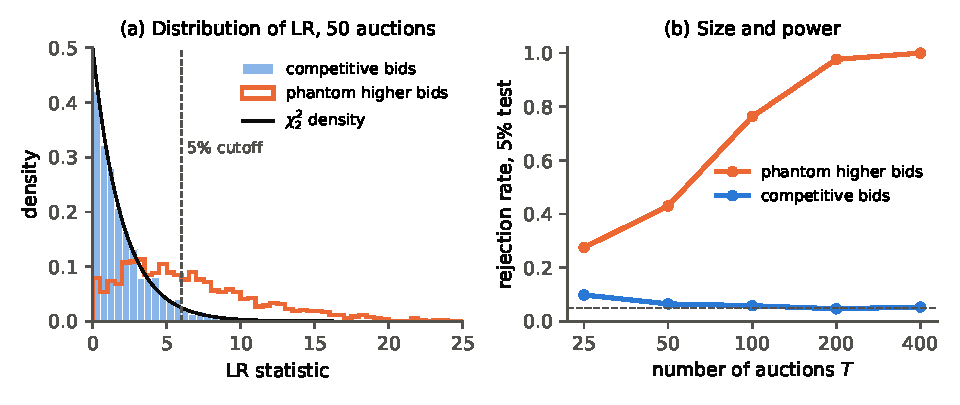
\includegraphics[width=\textwidth]{figures/ch13/pz_lr_sim.pdf}
\caption{Size and power of the rank-based test of \cref{cor:13-rank-lr} in simulated data. Panel (a) shows the
distribution of the likelihood ratio statistic over 2,000 samples of 50 auctions. The bars are for rankings that
follow the exploded logit, the line for rankings in which the nonwinning bids are in random order, and the curve is
the $\chi^2_2$ density. Panel (b) shows the rejection rates of the 5 percent test against the number of auctions,
with 600 samples per point. Our simulation, with sample sizes that mimic \citet{PorterZona1993}, Table~6.}
\label{fig:13-pz-sim}
\end{figure}

\subsection{Long Island highway paving: Porter and Zona (1993)}\label{sec:13-pz93}

\casehead{The question}
Can econometric tests detect a bid-rigging ring from public bid data when the ring includes only some of the
bidders? \citet{PorterZona1993} study contracts let by the New York State Department of Transportation (DOT) on
Long Island between April 1979 and March 1985. A group of firms bidding there was later named in bid-rigging suits.
The paper proposes test procedures and stresses their limits. In the authors' words, the tests ``will be poor
substitutes for a wiretap or a disclosure by a dissident ring member'' \citep[p.~1]{PorterZona1993}. They are,
however, better founded than the view that bid rotation or stable shares prove collusion.

\casehead{Institutional setting}
The DOT must award each highway contract to the lowest responsible bidder. It announces upcoming lettings in a
``Notice of Highway Lettings,'' and interested firms request plans and specifications. A ``Plan Buyers List'' of
the firms that bought plans for each job is distributed to subscribers, so each firm knows its potential rivals in
advance. On the day of the letting, sealed bids are opened and every bid and bidder is announced. The DOT checks
the low bid against its own cost estimate and then awards the contract. From April 1979 through March 1985 it
awarded about \$120 million of contracts in Nassau and Suffolk Counties, in 1969 dollars. There were 186 contracts,
161 of them below \$1 million. Sixty-six firms bid on at least one of the small contracts, but only 22 bid on jobs
above \$1 million. Four firms submitted 45 percent of the bids on those large jobs.

The authors list features of the market that facilitate collusion (WP pp.~8--12). The product is homogeneous,
because the contract defines the output, so a ring need only coordinate on price. Public announcement of bids and
bidders reveals any undercutting, and the plan buyers lists make the set of potential bidders common knowledge.
Demand was almost perfectly inelastic. With one exception, every contract was awarded to the low bidder whatever
the DOT's cost estimate, so any inflation of winning bids became profit. The exception is telling. In February
1983 the DOT solicited bids to resurface 0.8 miles of road, received eight bids with a low bid of about \$4 million,
and declined to award. When the job was rebid in May 1983, the low bid was 20 percent higher and came from the same
firm. A third letting in February 1984 drew three bids from firms that had bid both times before. The low bid was
about 10 percent above the second letting and 30 percent above the first, and the ranking of bidders never changed.
The contract had not been awarded by 1987.

Entry was difficult. Large jobs require batch concrete and asphalt plants, which incumbents owned, and newspaper
accounts report that union leaders discouraged outside bidders. Joint bids were allowed, which gave firms reasons to
communicate. Large jobs were let regularly, early each year, and usually one at a time. Such spacing limits what a
defector can earn before others retaliate. Firms bought inputs in the same markets, used the same technology and
employed members of the same unions, although backlogs and equipment differed.

\casehead{The candidate cartel}
In 1984 one of the five largest firms in the two counties was convicted in federal court of rigging bids on a Long
Island highway project that predates the sample. Four other firms were named as unindicted co-conspirators, and all
five were named in separate suits by New York State or Suffolk County. Each suit concerned a single job. The paper
treats these five firms, called Firms 2, 3, 4, 10 and 14, as a candidate ``cartel'' that may have operated in any
letting. The other bidders are called ``competitive.'' The cartel firms submitted 54 percent of the bids on larger
jobs and won 37 percent of all contracts. They also bid jointly at times (Table~1). Firms 4 and 2 did so in February
1980, with a winning bid of \$5.3 million. Firms 3 and 14 did so in June 1980 (\$7.3 million) and January 1982
(\$4.0 million), and Firms 3, 4 and 8 in November 1984 (\$8.0 million).

\Cref{tab:13-pz-cartel} shows that cartel firms regularly bid against each other on paving jobs. When Firm 2 bid,
another cartel firm also bid 88 percent of the time, and every bid by Firm 14 was accompanied by another cartel bid.
Insiders described the mechanism to a newspaper. Firms met around a conference table to review upcoming contracts
and decide ``who should get this one.'' Then ``the contractors who were tagged to be the low bidders would work out
their bid figures,'' and ``the rest of the contractors would then come up with higher bids'' \citep[p.~17]{PorterZona1993}.
Union representatives allegedly attended, communicated the low bids afterwards, and received a kickback of one percent of
the low bid on jobs won. This is a complementary bidding scheme, and the tests below are designed to detect it.

\begin{table}[htbp]
\centering
\caption{Bidding by the candidate cartel on Long Island paving jobs}\label{tab:13-pz-cartel}
\small
\begin{tabular}{@{}lccccc@{\hspace{2em}}cc@{}}
\toprule
 & \multicolumn{5}{c}{Bids also submitted by} & \multicolumn{2}{c}{Pr(another cartel bid), \%}\\
\cmidrule(lr){2-6}\cmidrule(l){7-8}
 & Firm 2 & Firm 3 & Firm 4 & Firm 10 & Firm 14 & Paving & Nonpaving\\
\midrule
Firm 2  & 48 & 37 & 34 & 1 & 11 & 88 & 75\\
Firm 3  & 37 & 86 & 56 & 1 & 15 & 79 & 55\\
Firm 4  & 34 & 56 & 71 & 2 & 14 & 89 & 80\\
Firm 10 & 1  & 1  & 2  & 3 & 1  & 67 & NA\\
Firm 14 & 11 & 15 & 14 & 1 & 20 & 100 & NA\\
\bottomrule
\end{tabular}

\smallskip
\begin{minipage}{0.92\textwidth}\footnotesize
Notes: Left panel, \citet{PorterZona1993}, Table~2: number of paving jobs on which the row firm and the column firm
both submitted individual bids. Diagonal entries are the row firm's total number of bids. Joint bids are excluded.
Right panel, Table~3: percentage of the row firm's bids on which at least one other cartel firm also bid. NA: not
available. NBER working-paper version.
\end{minipage}
\end{table}

\casehead{Two conventional indicators}
The first indicator is the stability of market shares. On paving jobs the cartel firms' annual shares varied
substantially, and Firm 10 stopped bidding early in the sample (it bid only three times). No pattern of rotation is
apparent. Newspaper accounts nonetheless report stable shares in state highway and sewer work for more than a
decade, on many jobs outside the sample. Shares on paving alone would thus give an unwarranted impression of
competition.

The second indicator is the dispersion of bids within a job. The 116 paving jobs received 347 competitive bids on
103 jobs and 228 cartel bids on 109 jobs. On the 76 jobs with at least two cartel bids, the second-lowest cartel bid
exceeded the lowest by 4.96 percent on average, measured as the mean difference in log bids. On the 75 jobs with at
least two competitive bids, the corresponding figure is 6.25 percent. Competitive bids are more numerous per job,
and \cref{ex:13-gap-uniform} shows that more bids shrink the expected gap. The comparison therefore understates
how much tighter the cartel bids are. The pattern resembles the clustering found by \citet{FeinsteinBlockNold1985}
in North Carolina highway contracts.

\casehead{Data}
The analysis uses contracts that involve paving, where the facilitating features are strongest. Mowing, painting
and traffic signal contracts are excluded. The 116 paving projects received 575 bids. Joint bids, under 2 percent of
paving bids, are dropped. Estimating the auction-specific variance $\sigma_t^2$ requires at least two competitive
bids, which leaves 75 projects with 319 competitive bids and 157 cartel bids.

The covariates measure cost differences across firms. $\mathit{BACKLOG}_{it}$ is the dollar value of DOT contracts
that firm $i$ has won but not completed, assuming completion at a constant pace over about three months. Capacity is
the largest backlog the firm carried in the sample, $\mathit{CAP}_i = \max_t \mathit{BACKLOG}_{it}$, and enters with
its square $\mathit{CAPSQ}$. $\mathit{NOBACK}$ marks noncartel firms that never won, for which $\mathit{CAP} = 0$.
Utilization is $\mathit{UTIL}_{it} = \frac{\mathit{BACKLOG}_{it}}{\mathit{CAP}_i}$ (zero when $\mathit{CAP}_i = 0$),
and enters with its square $\mathit{UTILSQ}$. $\mathit{ISLAND}$ marks firms headquartered on Long Island, which
includes all cartel firms. No job-specific data are available, not even the engineers' estimates. The dependent
variable is the log bid, in hundreds of thousands of 1969 dollars. The mean competitive bid was \$450,000 and the mean
cartel bid \$713,000.

\casehead{Model and estimating equations}
The competitive model is \cref{asm:13-competitive-bidding}, with cost distributions allowed to differ across firms
and jobs. Equilibrium bids satisfy \eqref{eq:13-proc-foc}, and the bid rule \eqref{eq:13-pz-bid} approximates the
equilibrium bid function. It imposes two restrictions. Firms respond in the same way to the observed covariates, and
all job-level heterogeneity is captured by the auction effect $\alpha_t$. The authors emphasize between-firm rather
than between-job variation because they have no job characteristics.

The bid levels are estimated by feasible generalized least squares in two steps. First, ordinary least squares on
the competitive bids, with a dummy for each auction, gives residuals $\hat\epsilon_{it}$. The auction variance is
estimated by the mean squared residual of the competitive bids in that auction,
\begin{equation}\label{eq:13-pz-sigma}
  \hat\sigma_t^2 = \frac{1}{n^{c}_t}\sum_{i \in \mathcal{N}^{c}_t}\hat\epsilon_{it}^{\,2},
\end{equation}
where $\mathcal{N}^c_t$ is the set of $n^c_t$ competitive bidders. Second, every observation is divided by
$\hat\sigma_t$ and the auction-dummy regression is run again. The same weights are used for three samples: all
bids, competitive bids, and cartel bids. If all bids are competitive, the three regressions estimate the same
$\beta$. If cartel bids are not competitive, only the competitive regression is consistent. A Chow test compares
the pooled regression with the two separate ones.

The rank analysis applies \cref{prop:13-exploded-logit} with $Z_{it} = -\frac{x_{it}}{\hat\sigma_t}$. It is run
separately on the ranking of competitive bids and on the ranking of cartel bids among themselves. Within each
group, the coefficients are estimated from all ranks, from the lowest rank only and from the higher ranks only,
and \cref{cor:13-rank-lr} gives the test.

\casehead{Identification}
Within an auction, bidders differ in backlog, capacity and location, and this variation identifies $\beta$. The
auction effects absorb the size, type and location of the job, which are unobserved. The rank likelihood removes
them altogether. The test for collusion rests on an asymmetry between cartel bids. A designated cartel winner must
still beat the outsiders, so it trades a higher margin against a lower probability of winning, as a competitive
bidder does. Complementary bids are designed to lose and need not respond to costs. Under phantom bidding, the
determinants of the lowest cartel bid should therefore differ from those of the higher cartel bids. The same test
applied to competitive bids is a placebo. Passing it makes it less likely that the model omits a variable that
affects high and low bids differently. The test is agnostic about how the ring chooses its winner.

\casehead{Results: bid levels}
\Cref{tab:13-pz-t4} reproduces the generalized least squares estimates. The competitive model fits well. The Wald
statistic for the six covariates is 494.7, against a $\chi^2_6$ distribution. Long Island firms bid about 3 percent
less than other firms, although the coefficient is imprecise. Bids first fall and then rise with utilization. The
effect of utilization $u$ on the log bid is $-0.0973u + 0.1720u^2$. It equals $-0.014$ at $u = 0.3$ and $0.075$ at
full capacity, and it reaches its minimum at $u = 0.28$ (our computation). These values match the paper's
statements that bids are about 1.5 percent lower at 30 percent utilization and 7.5 percent higher at full capacity. Bids also fall and then rise
with capacity, with only one firm beyond the minimum.

\begin{table}[htbp]
\centering
\caption{Generalized least squares estimates of the log bid equation, Long Island paving}\label{tab:13-pz-t4}
\small
\begin{tabular}{@{}lccc@{}}
\toprule
 & All firms & Competitive firms & Cartel firms\\
\midrule
$\mathit{UTIL}$   & $-0.0053$ & $-0.0973$ & $0.1991$\\
                  & (0.2) & (2.8) & (1.2)\\
$\mathit{UTILSQ}$ & $0.0358$ & $0.1720$ & $-0.1143$\\
                  & (1.0) & (4.0) & (0.8)\\
$\mathit{NOBACK}$ & $-0.0010$ & $-0.0178$ & \\
                  & (0.1) & (1.6) & \\
$\mathit{CAP}$    & $0.1666$ & $-1.2691$ & $1.8225$\\
                  & (1.8) & (10.4) & (4.6)\\
$\mathit{CAPSQ}$  & $-0.4430$ & $4.8519$ & $-2.9029$\\
                  & (2.1) & (13.0) & (4.4)\\
$\mathit{ISLAND}$ & $-0.0288$ & $-0.0334$ & \\
                  & (0.6) & (1.2) & \\
\midrule
Observations       & 476 & 319 & 157\\
Degrees of freedom & 395 & 238 & 81\\
Wald statistic     & 21.9 & 494.7 & 28.4\\
\bottomrule
\end{tabular}

\smallskip
\begin{minipage}{0.86\textwidth}\footnotesize
Notes: Reproduced from \citet{PorterZona1993}, Table~4 (NBER working-paper version). Absolute values of
$t$-statistics in parentheses, as in the paper. Auction-specific constants included but not reported. All
regressions use the auction variance weights estimated from competitive bids. Coefficients of $\mathit{CAP}$ and
$\mathit{CAPSQ}$ are scaled up by $10^4$ and $10^8$. $\mathit{NOBACK}$ and $\mathit{ISLAND}$ are not identified for
cartel firms. The Wald statistic tests the joint significance of the reported coefficients.
\end{minipage}
\end{table}

The cartel estimates look very different. Utilization enters with the opposite curvature, and capacity enters
with the opposite signs, significantly so. Many cartel coefficients do not have the expected sign. The Chow test
statistic is $F(76, 319) = 9.38$, with a $p$-value below $10^{-40}$ (our computation), so bids from cartel firms
differ statistically from competitive bids. The degrees of freedom reveal what the test compares. The denominator,
319, is the sum of the residual degrees of freedom of the two separate regressions, $238 + 81$. The numerator, 76,
equals the 4 cartel slopes plus 72 cartel auction constants (our reading of Table~4). The Chow test therefore
compares the levels of cartel and competitive bids within auctions as well as their slopes.

\casehead{Results: bid ranks}
\Cref{tab:13-pz-tests} reproduces the rank-based estimates. For competitive bids, the estimates are stable across
ranks. Capacity matters with similar coefficients in the lowest rank and in the higher ranks ($-1.641$ and $-2.100$
for $\mathit{CAP}$, 6.517 and 7.020 for $\mathit{CAPSQ}$). The likelihood ratio statistic is
\begin{equation*}
  LR^{\mathrm{comp}} = 2\,\bigl[-89.85 - 199.4 - (-291.4)\bigr] = 4.30 ,
\end{equation*}
against a $\chi^2_6$ distribution, with $p = 0.64$ (our computation). The paper reports that the statistic ``is
significant at about the 36 percent level,'' which is the value of the $\chi^2_6$ distribution function. Competitive
bids appear to be generated by the same process whether or not they are low.

\begin{table}[htbp]
\centering
\caption{Rank-ordered logit estimates for competitive and cartel bids, Long Island paving}\label{tab:13-pz-tests}
\small
\setlength{\tabcolsep}{5pt}
\begin{tabular}{@{}lcccccc@{}}
\toprule
 & \multicolumn{3}{c}{Competitive bids (Table~5)} & \multicolumn{3}{c}{Cartel bids (Table~6)}\\
\cmidrule(lr){2-4}\cmidrule(l){5-7}
 & All ranks & Low rank & Higher ranks & All ranks & Low rank & Higher ranks\\
\midrule
$\mathit{UTIL}$   & $-0.0070$ & $0.0161$ & $-0.0522$ & $0.0429$ & $0.2107$ & $0.2310$\\
                  & (0.1) & (0.1) & (0.3) & (0.3) & (1.0) & (0.6)\\
$\mathit{UTILSQ}$ & $0.0986$ & $0.0534$ & $0.1596$ & $-0.0112$ & $-0.1128$ & $-0.4300$\\
                  & (0.8) & (0.3) & (1.0) & (0.1) & (0.6) & (0.9)\\
$\mathit{NOBACK}$ & $-0.0283$ & $0.0089$ & $-0.0454$ & & & \\
                  & (1.0) & (0.2) & (1.3) & & & \\
$\mathit{CAP}$    & $-1.888$ & $-1.641$ & $-2.100$ & $0.4306$ & $1.101$ & $-2.537$\\
                  & (3.8) & (2.4) & (3.0) & (0.9) & (1.3) & (1.6)\\
$\mathit{CAPSQ}$  & $6.869$ & $6.517$ & $7.020$ & $-0.8473$ & $-1.904$ & $3.861$\\
                  & (3.9) & (2.6) & (2.9) & (0.9) & (1.2) & (1.4)\\
$\mathit{ISLAND}$ & $-0.0182$ & $-0.0759$ & $0.1016$ & & & \\
                  & (0.3) & (0.9) & (0.9) & & & \\
\midrule
Choice sets    & 244 & 75 & 169 & 85 & 50 & 35\\
Log likelihood & $-291.4$ & $-89.85$ & $-199.4$ & $-73.97$ & $-44.58$ & $-24.92$\\
LR test & \multicolumn{3}{c}{4.30 ($\chi^2_6$), $p = 0.64$} & \multicolumn{3}{c}{8.94 ($\chi^2_4$), $p = 0.063$}\\
\bottomrule
\end{tabular}

\smallskip
\begin{minipage}{0.95\textwidth}\footnotesize
Notes: Reproduced from \citet{PorterZona1993}, Tables~5 and~6 (NBER working-paper version). Absolute
$t$-statistics in parentheses. Coefficients of $\mathit{CAP}$ and $\mathit{CAPSQ}$ scaled up by $10^4$ and $10^8$. A
choice set is one factor of \eqref{eq:13-rank-likelihood}: an auction with $n$ ranked bids contributes one low-rank
and $n-2$ higher-rank choice sets. The $p$-values are our computation from the reported statistics.
\end{minipage}
\end{table}

For cartel bids the picture changes. The likelihood ratio statistic is
\begin{equation*}
  LR^{\mathrm{cartel}} = 2\,\bigl[-44.58 - 24.92 - (-73.97)\bigr] = 8.94 ,
\end{equation*}
against a $\chi^2_4$ distribution, because $\mathit{NOBACK}$ and $\mathit{ISLAND}$ are not identified. The $p$-value
is 0.063 (our computation), which the paper describes as significance ``at about the 94 percent level.'' The authors
reject the null hypothesis of no phantom bidding and conclude that cartel bids are generated by a different process
depending on whether they are low or not. The bookkeeping of the samples is informative. The 85 cartel choice sets
come from 50 auctions with two or more cartel bids, so these auctions contain 135 cartel bids, and only 35 choices
inform the higher-rank coefficients (our computation).

Two further features of the estimates deserve attention. The cartel rank estimates resemble the cartel bid-level
estimates of \cref{tab:13-pz-t4} and differ from all the competitive estimates. The two methods are also mutually
consistent for competitive bids. Under \eqref{eq:13-rank-index} the rank coefficients should equal
$\frac{\pi}{\sqrt6} \approx 1.28$ times the bid-equation coefficients. Scaled by this factor, the
competitive estimates of $\mathit{CAP}$ and $\mathit{CAPSQ}$ in \cref{tab:13-pz-t4} are $-1.63$ and 6.22 (our
computation). Given their standard errors, they are close to the rank estimates of $-1.89$ and 6.87. The small
utilization coefficients fail this check, but they are imprecise in the rank model.

\casehead{Robustness}
The paper reports few robustness checks beyond the competitive-rank test, which serves as a specification check.
The agreement between bid-level and rank-based results for each group of firms is a second check. The authors argue
that their classification is conservative. If some ring members were classified as competitive, the competitive
benchmark would be contaminated, which works against finding a difference.

\casehead{Interpretation}
Competitive bids are related to backlog and capacity at every rank, as cost-based bidding requires. The ranking of
the higher cartel bids does not reflect the same cost measures, and it differs from the determinants of the lowest
cartel bid. This is the footprint of complementary bids that are designed to lose. Together with the frequency of
cartel firms bidding against one another and the tight clustering of their bids, the evidence fits the scheme that
insiders described. The authors conclude that, since they have no reason to believe the difference is structural,
they ``may have found evidence of cartel activity'' \citep[p.~36]{PorterZona1993}.

\casehead{Critiques and limitations}
Several limitations follow from the design.
\begin{enumerate}[label=(\arabic*)]
\item Ring membership is not random. Cartel firms were larger, with a mean bid of \$713,000 against \$450,000, and
all were based on Long Island. Their bids could differ for structural reasons. The passing competitive-rank test
argues against general misspecification, but it cannot rule out effects specific to these firms.
\item The rank test is weak. The rejection relies on 35 higher-rank choices and has a $p$-value of 0.063. The
simulation in \cref{fig:13-pz-sim} suggests a power of about one half at this sample size even when the higher bids
ignore costs entirely.
\item The weights and standardized regressors use $\hat\sigma_t$, estimated in some auctions from just two
competitive bids. The reported standard errors do not account for this first step.
\item The covariates are crude. Backlog assumes three-month completion, there are no job characteristics, and the
model assumes independent private costs with a common response to the covariates.
\item The designated winner need not be the lowest-cost member. The cartel low-rank coefficients on capacity have
signs opposite to the competitive ones, although they are imprecise. This is consistent with a winner chosen by
turns or by equity criteria (our reading). The test remains valid in that case, because it only requires the higher
bids to be uninformative about costs.
\item A ring can adapt. If the procedure were announced, an effective cartel could scale all its bids by a common
factor, so that its ranking matches cost rankings. A noninclusive ring would then look like a group of firms with
different costs \citep[p.~36]{PorterZona1993}. \citet[pp.~246--247]{MarshallMarx2012} make the same point. They
call the rank test a plus factor that is not substantive, because a ring can alter its losing bids at no cost to
its mechanism (\cref{sec:13-market-evidence}).
\end{enumerate}

\casehead{Contribution}
The paper turned the detection of bid rigging into a problem of testing a competitive model against a specific
footprint of collusion. Its central idea is that designated and complementary bids obey different economic logic,
and that firms outside the ring provide a benchmark for the competitive model. The rank-ordered logit lets the
test ignore unobserved job characteristics. Later work, including \citet{PorterZona1999} and \citet{BajariYe2003},
follows the same logic of a competitive model, a control group and scheme-specific restrictions.
\Cref{ch:auction-empirics} returns to tests for collusion based on structural auction models.

\subsection{Ohio school milk: Porter and Zona (1999)}\label{sec:13-pz99}

\casehead{The question}
Did dairies around Cincinnati collude in school milk auctions in the 1980s, and by how much did collusion raise the
prices paid by school districts? In \emph{State of Ohio v.\ Louis Trauth Dairy, Inc., et al.}, the State charged
thirteen dairies with collusion in school milk auctions from 1980 through 1990. The case settled before trial.
\citet{PorterZona1999} adapt their reports for the plaintiff. Unlike the Long Island data, the Ohio data describe the
districts and the contract terms, so both the decision to bid and the level of the bid can be modeled.

\casehead{Setting}
Ohio has more than 600 school districts. Each district solicits bids between May and August for the supply of milk
in half pints during the next school year. A district might announce, for example, that it expects to buy 50,000 half
pints of whole white milk and 30,000 of whole chocolate milk, enough for about 450 students. Bidders submit a list of
prices, and the district may require coolers, straws or napkins, or allow escalator clauses that index prices to raw
milk. The low bidder usually wins.

Demand is insensitive to price. Using 609 districts in May 1990, the authors regress the log of half pints bought on
log enrollment and the log of the standardized price (WP p.~6, footnote 4). The estimates are
\begin{equation*}
  \ln q = 2.69 + 1.029 \ln(\text{enrollment}) + 0.21 \ln(\text{price}), \qquad R^2 = 0.84 .
\end{equation*}
The $t$-statistics on the slopes are 56.6 and 1.4, so price has no significant effect. A firm that controls supply to a
district can therefore command a much higher price there.

Costs are similar across dairies apart from distance. Raw milk prices are regulated by location and type, and the
raw milk in a half pint costs about seven cents. Packaging costs about two cents and delivery about one cent, so total
incremental cost is about ten cents per half pint (WP pp.~6--9). A cooler adds about 0.2 cents. Suppliers are
processors, which pasteurize and package milk, or distributors, which buy from processors. School milk is under 10
percent of processors' revenues, and no plant was built to serve schools alone. Transport costs and regulation make
competition local.

\casehead{Facilitating features and the testimony}
The paper lists many features that facilitate collusion (WP pp.~10--13). Firms compete only on price, bids and
bidders are announced, and districts let contracts at different times. Staggered lettings let a ring adjust its
allocation during the season and retaliate almost at once. Demand is predictable, district boundaries make
territories easy to define, and the set of potential bidders is small and stable. Dairies meet in many markets,
which by \citet{BernheimWhinston1990} relaxes the incentive constraints that limit collusion. Firms obtained rivals'
price lists through grocery customers, dairies bought from one another, and trade associations met regularly. Price
decks assigned districts to a few price levels, and one level could serve for complementary bids.

In 1993 representatives of two dairies in southwestern Ohio confessed to rigging bids during the sample period. The
paper later identifies their testimony as that of Meyer and Coors (WP p.~28). They described a scheme of respecting
incumbency. If a cartel member had served a district the previous year, the others submitted high complementary
bids that would not undercut it, or did not bid. The specific arrangements were worked out through frequent
communication during each bidding season. The witnesses also testified that the cartel broke down in two school
years, 1983--84 and 1989--90. The authors note that territorial assignment would be the more practical scheme for
firms that are far apart.

\casehead{Data}
The State of Ohio collected bid data for as many as 509 of the roughly 600 districts from 1980 through 1990, with
about 60 bidders at some point in the sample. \Cref{tab:13-pz99-t1} summarizes the data. Of 68 processing plants
with sales in Ohio during the period, 46 supplied school milk in 1987. A map of these plants (Figure~1 of the paper)
shades areas by the concentration of plant ownership within 75 miles. The northeast is least concentrated, and
Columbus and the southern tip of the state are most concentrated. The number of plants serving districts fell from
54 to 43 between 1980 and 1990, and the number of bidding dairies from 43 to 26.

\begin{table}[htbp]
\centering
\caption{The Ohio school milk data, 1980--1990}\label{tab:13-pz99-t1}
\small
\begin{tabular}{@{}lrrrrcc@{}}
\toprule
Year & Districts & Enrollment & Plants & Dairies & Average price & Raw milk price\\
\midrule
1980 & 366 & 1,257,925 & 54 & 43 & 0.12823 & 0.0718\\
1981 & 398 & 1,379,619 & 50 & 44 & 0.12950 & 0.0769\\
1982 & 415 & 1,371,164 & 46 & 40 & 0.12954 & 0.0760\\
1983 & 436 & 1,415,281 & 48 & 40 & 0.12883 & 0.0764\\
1984 & 448 & 1,430,644 & 53 & 38 & 0.13133 & 0.0741\\
1985 & 463 & 1,460,697 & 48 & 35 & 0.13215 & 0.0708\\
1986 & 481 & 1,457,437 & 47 & 36 & 0.13042 & 0.0700\\
1987 & 494 & 1,566,591 & 46 & 33 & 0.13099 & 0.0701\\
1988 & 509 & 1,520,635 & 44 & 30 & 0.13378 & 0.0666\\
1989 & 491 & 1,564,869 & 43 & 26 & 0.13886 & 0.0708\\
1990 & 412 & 1,296,587 & 43 & 26 & 0.15751 & 0.0797\\
\bottomrule
\end{tabular}

\smallskip
\begin{minipage}{0.92\textwidth}\footnotesize
Notes: Reproduced from \citet{PorterZona1999}, Table~1 (NBER working-paper version). Districts: school
districts or cooperatives in the data. Enrollment: total enrollment in those districts. Plants: plants operated by
submitting dairies. Dairies: dairies submitting bids. Prices in dollars per half pint. The raw milk price is the
July Federal Milk Order No.~33 Class~I price, converted at 186 half pints per hundredweight.
\end{minipage}
\end{table}

Distance shapes participation. A non-defendant firm bids on 19.5 percent of the districts within 10 miles of its
plant (Table~2). The probability falls to 7.6 percent at 20 to 30 miles, 2.3 percent at 40 to 50 miles and 0.5
percent at 100 to 150 miles. The probability of winning is 13.6 percent within 10 miles. These figures
come from 2,053 bids out of 73,965 bid opportunities, of which 1,260 won. About 85 percent of suppliers serve
districts from plants less than 75 miles away. Few firms bid in any auction (Table~3). Of 3,866 auctions, 45.0
percent drew one bidder, 33.6 percent two and 18.2 percent three, with a mean of 1.8. The firm with the plant
closest to the district submitted 42.8 percent of the 6,965 bids and won 48.8 percent of the 3,511 contracts
(Table~4).

\casehead{The competitive model: bid submission}
Non-defendant firms form the \emph{control group}, whose behavior defines the competitive benchmark. A competitive
dairy decides where to bid and how much to bid. Let $d$ index districts and $t$ years. The submission decision of
firm $i$ is a probit,
\begin{equation}\label{eq:13-pz99-probit}
  S^*_{idt} = w_{idt}\gamma + u_{idt}, \qquad S_{idt} = \indic\{S^*_{idt} > 0\}, \qquad u_{idt} \sim N(0,1) .
\end{equation}
The covariates $w_{idt}$ include distance from the firm's nearest plant to the district, and a processor dummy and
its interactions. They include $\mathit{Direction}$, the share of the firm's bids placed in the quadrant where the
district lies, which proxies for route structure. They also include $\mathit{Size}$, the firm's share of Ohio
students served, dummies for the closest and second-closest plants, district enrollment, contract terms and year
effects. Three
specifications are estimated: pooled, with bidder fixed effects, and with bidder and district fixed effects. The
last has over 400 coefficients and is estimated on two halves of the districts. Its distance coefficient is
identified because plant closures change distances over time.

\Cref{tab:13-pz99-control} reports selected estimates. Processors bid more often than distributors. Distance sharply
lowers the probability of bidding, more so for processors. Firms bid more often in the direction of their existing
routes, and the closest firm is more likely to bid. \Cref{fig:13-pz99-f2} plots the predicted probability of bidding
by distance for a hypothetical control-group processor. The probability starts near or above one half at zero
distance and steps down where the firm loses its locational advantage. It is close to zero beyond 75 miles.

\casehead{The competitive model: bid levels and selection}
The bid variable is a summary price per half pint for two-percent chocolate milk. Each submitted price for another
type of milk is converted with a pairwise regression, for example of chocolate on white milk prices, and the
predictions are averaged. The bid equation is
\begin{equation}\label{eq:13-pz99-bid}
  b_{idt} = x_{idt}\beta + e_{idt}, \qquad b_{idt} \text{ observed only if } S_{idt} = 1 ,
\end{equation}
with $(e_{idt}, u_{idt})$ independent of the regressors $(x_{idt}, w_{idt})$ and bivariate normal with mean zero,
$\Var(e_{idt}) = \sigma_e^2$, $\Var(u_{idt}) = 1$ and correlation $\varrho$. The conditional distribution of the
errors given the regressors is then this fixed bivariate normal. Bids are observed only for firms that chose to bid,
so ordinary least squares on submitted bids is biased if $\varrho \neq 0$.

\begin{lemma}[Selection correction]\label{lem:13-heckman}
In the model \eqref{eq:13-pz99-probit}--\eqref{eq:13-pz99-bid},
\begin{equation}\label{eq:13-heckman}
  \E\bigl[b_{idt} \mid x_{idt}, w_{idt}, S_{idt} = 1\bigr] = x_{idt}\beta + \varrho\,\sigma_e\,\lambda(w_{idt}\gamma),
  \qquad \lambda(z) = \frac{\phi(z)}{\Phi(z)} ,
\end{equation}
where $\phi$ and $\Phi$ are the standard normal density and distribution function, and $\lambda$ is the
\emph{inverse Mills ratio}.
\end{lemma}

\begin{proof}
Condition on $(x, w)$ throughout. Since the errors are independent of the regressors, the pair $(e, u)$ keeps its
bivariate normal distribution given $(x, w)$. For a bivariate normal pair with mean zero and $\Var(u) = 1$, the
regression of $e$ on $u$ is linear, $\E[e \mid u] = \varrho\sigma_e u$. Since $S = 1$ exactly when $u > -w\gamma$,
iterated expectations give
$\E[e \mid u > -w\gamma] = \varrho\sigma_e\,\E[u \mid u > -w\gamma]$. Write $a = w\gamma$. Using $\phi'(u) = -u\phi(u)$,
\begin{equation*}
  \E[u \mid u > -a] = \frac{\int_{-a}^{\infty}u\,\phi(u)\,du}{1 - \Phi(-a)}
  = \frac{\bigl[-\phi(u)\bigr]_{-a}^{\infty}}{\Phi(a)} = \frac{\phi(-a)}{\Phi(a)} = \frac{\phi(a)}{\Phi(a)} ,
\end{equation*}
where the last two steps use the symmetry of the normal distribution. Adding $x\beta$ gives \eqref{eq:13-heckman}.
\end{proof}

The two-step estimator of \citet{Heckman1979} estimates the probit, forms $\hat\lambda_{idt} = \lambda(w_{idt}\hat\gamma)$,
and regresses submitted bids on $x_{idt}$ and $\hat\lambda_{idt}$. The coefficient on $\hat\lambda$ estimates
$\varrho\sigma_e$ (\cref{app:econometrics}). Identification does not rest on the normal functional form alone,
because several probit regressors are excluded from the bid equation. Comparing Tables~6 and~7 of the paper,
$\mathit{Direction}$ and its interactions, $\mathit{Size}$ and its interactions, and the second-closest dummy shift
participation but not the bid. Route structure and scale plausibly affect the cost of adding a district to a delivery
schedule, and hence the decision to bid, more than the bid itself. This exclusion is nonetheless an assumption.

\begin{table}[htbp]
\centering
\caption{The competitive benchmark: control-group submission and bid equations}\label{tab:13-pz99-control}
\small
\begin{tabular}{@{}lcccc@{}}
\toprule
 & \multicolumn{2}{c}{Base model} & \multicolumn{2}{c}{Bidder fixed effects}\\
\cmidrule(lr){2-3}\cmidrule(l){4-5}
 & Coefficient & $t$ & Coefficient & $t$\\
\midrule
\multicolumn{5}{@{}l}{\textit{Panel A. Probit for bid submission (Table~6)}}\\
Distance                      & $-0.015453$ & $-10.1$ & $-0.022971$ & $-12.4$\\
Processor                     & 1.778220 & 18.6 & 1.689650 & 10.4\\
Processor $\times$ Distance   & $-0.035257$ & $-15.4$ & $-0.047488$ & $-13.2$\\
Direction                     & 1.146110 & 16.1 & 1.272590 & 15.5\\
Direction $\times$ Distance   & 0.005570 & 3.6 & 0.013020 & 7.0\\
Size                          & 27.876500 & 17.0 & 12.202800 & 4.6\\
Closest                       & 0.370670 & 9.9 & 0.329990 & 7.3\\
Second closest                & 0.089160 & 1.6 & 0.189010 & 3.0\\
District enrollment           & $-0.000013$ & $-4.2$ & $-0.000011$ & $-3.4$\\
Log likelihood                & \multicolumn{2}{c}{$-5964$} & \multicolumn{2}{c}{$-5052$}\\
Observations (parameters)     & \multicolumn{2}{c}{73,965 (25)} & \multicolumn{2}{c}{73,965 (89)}\\
\midrule
\multicolumn{5}{@{}l}{\textit{Panel B. Bid level with selection correction, dollars per half pint (Table~7)}}\\
Constant                      & 0.123542 & 59.5 & 0.128517 & 33.9\\
Distance                      & 0.000027 & 2.3 & 0.000004 & 0.3\\
Processor $\times$ Distance   & 0.000009 & 0.6 & 0.000065 & 2.9\\
Processor                     & $-0.002200$ & $-3.1$ & $-0.001300$ & $-0.7$\\
Closest                       & 0.003535 & 4.1 & 0.000494 & 0.6\\
Closest $\times$ Distance     & $-0.000069$ & $-2.3$ & $-0.000002$ & $-0.1$\\
Inverse Mills ratio           & 0.001713 & 2.9 & 0.001586 & 2.6\\
Fixed bid                     & 0.002334 & 3.1 & 0.001174 & 2.0\\
Escalator                     & $-0.003030$ & $-3.5$ & $-0.000890$ & $-1.3$\\
Year 1990                     & 0.031683 & 31.0 & 0.032510 & 36.1\\
$R^2$ (RMSE)                  & \multicolumn{2}{c}{0.4891 (0.009540)} & \multicolumn{2}{c}{0.7337 (0.007000)}\\
Observations                  & \multicolumn{2}{c}{2,053} & \multicolumn{2}{c}{2,053}\\
\bottomrule
\end{tabular}

\smallskip
\begin{minipage}{0.92\textwidth}\footnotesize
Notes: Selected rows of \citet{PorterZona1999}, Tables~6 and~7, columns (a)--(d) (NBER working-paper version). Signed $t$-statistics as in the paper. Both equations also include contract terms, delivery and
cooperative variables, and the bid equation includes year effects for 1981--1990. The tables also report a
specification with bidder and district fixed effects with similar coefficients of interest. The inverse Mills ratio
in each bid equation uses the corresponding probit.
\end{minipage}
\end{table}

Panel B of \cref{tab:13-pz99-control} shows the bid results. The coefficient on the inverse Mills ratio is positive.
Since $\lambda$ falls as the probability of bidding rises, firms that are likely to submit a bid tend to bid low.
Bids rise with distance. Table~8 of the paper reports the derivative of the predicted bid with respect to distance,
including the effect that runs through the selection term. For a firm that is not the closest supplier, the base
model gives 0.0096 dollars per half pint per hundred miles. The specifications with bidder effects and with bidder
and district effects give 0.0154 and 0.0194. The direct distance coefficients in column (a) imply only 0.0036 dollars per hundred miles for
a processor (our computation). Most of the base-model gradient therefore appears to work through selection (our
reading). As distance rises, the probability of bidding falls, $\lambda$ rises and the predicted bid rises with it. \Cref{fig:13-pz99-f3} plots
the predicted bid against distance. A bid 100 miles away is over a penny higher than a bid next to the plant.
Moderate increases in distance raise bids by about ten percent (WP pp.~20 and~24). With bidder effects, an escalating
bid is about 0.2 cents lower than a fixed bid ($0.001174 + 0.000890$). The 1990 year effect of about three cents
reflects the jump in the raw milk price that year (\cref{tab:13-pz99-t1}).

\begin{figure}[htbp]
\centering
\begin{subfigure}{0.78\textwidth}
\centering
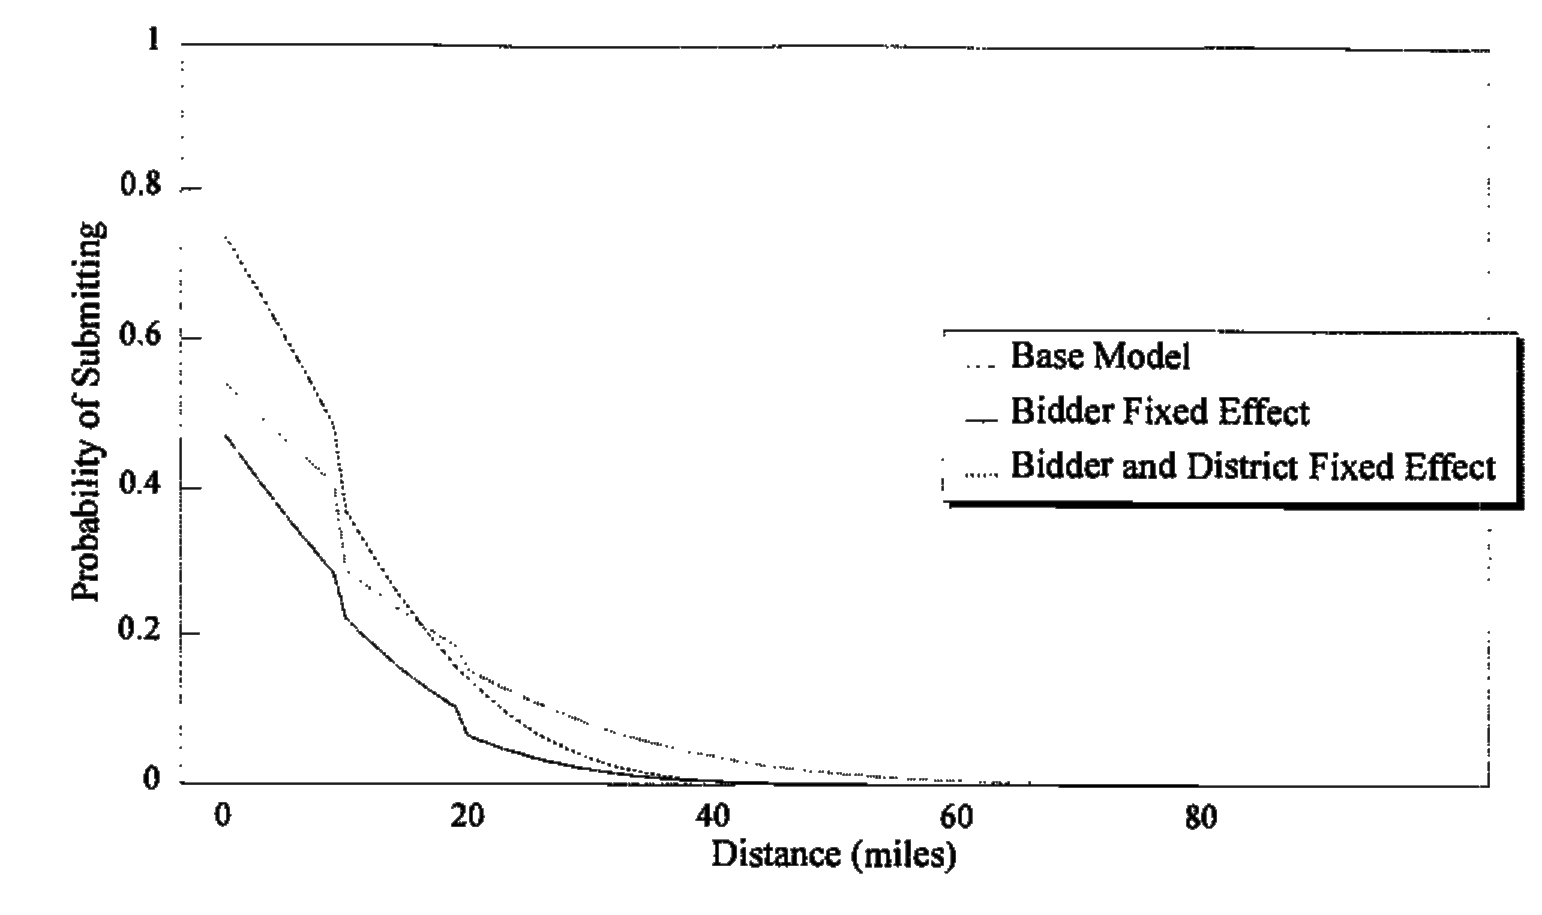
\includegraphics[width=\textwidth]{figures/ch13/pz99_fig2.png}
\caption{Predicted probability of submitting a bid}\label{fig:13-pz99-f2}
\end{subfigure}

\medskip
\begin{subfigure}{0.78\textwidth}
\centering
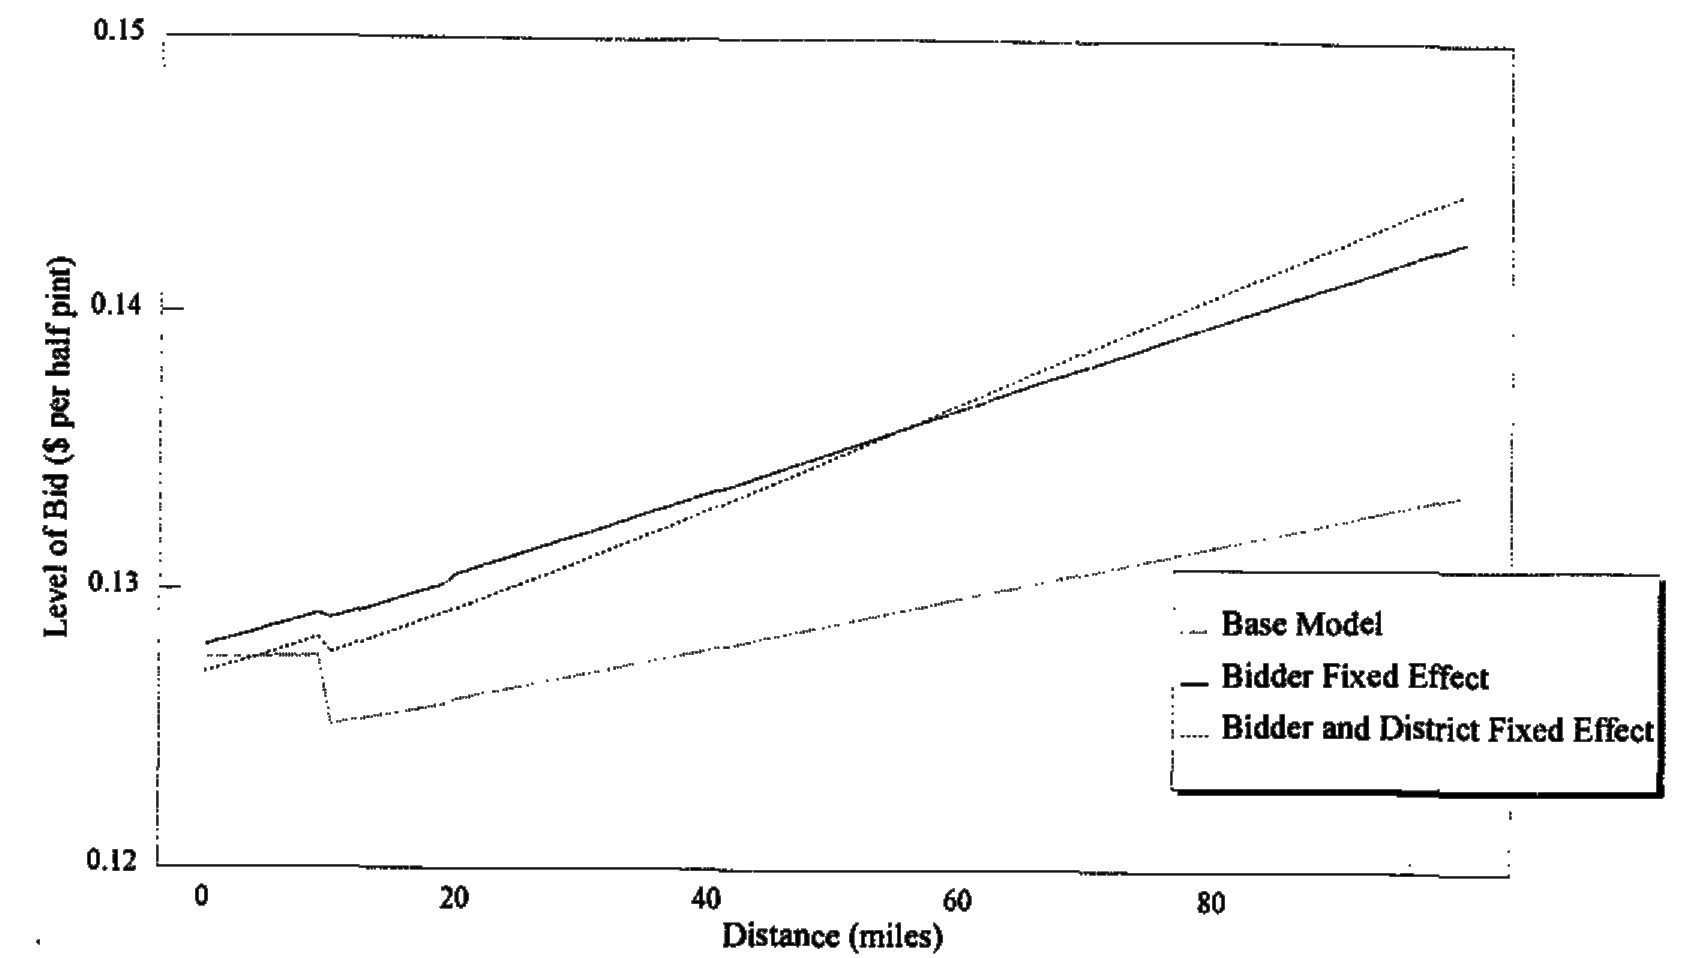
\includegraphics[width=\textwidth]{figures/ch13/pz99_fig3.png}
\caption{Predicted level of submitted bids, dollars per half pint}\label{fig:13-pz99-f3}
\end{subfigure}
\caption{The competitive benchmark in Ohio school milk: predictions for a hypothetical control-group processor by
distance from its plant, under the three specifications. Variables unrelated to distance are at their means, the
firm is the closest supplier within 10 miles and the second closest between 10 and 20 miles. The steps occur where
the firm loses these positions. The bidder fixed-effects curves are solid. In panel (a) the base model is the dotted
curve with the longest tail, and in panel (b) it is the lowest curve beyond 10 miles. The scans are darkened for
legibility. Source: \citet{PorterZona1999}, Figures~2 and~3 (NBER working-paper version).}
\label{fig:13-pz99-f23}
\end{figure}

The authors conclude that the control group bids in a way consistent with competition in a spatial market where
each firm has some local market power. Bids rise with distance, and firms rarely bid far from their plants.

\casehead{Defendants versus the control group}
The paper studies six southwestern Ohio defendants: Beatrice, Borden, Coors Brothers, H.~Meyer, Louis Trauth and
Meadow Gold. Beatrice and Meadow Gold are the same firm bidding under two names. Two tests ask whether each defendant
follows the control-group model.

The first test concerns submission. For each defendant, the authors append its submission data to the control-group
data and estimate the probit twice. Under the null hypothesis the defendant shares the control group's slopes but
has its own intercept. Under the alternative it has its own slopes. The likelihood ratio statistic is
$2(\ell^{\mathrm{alt}} - \ell^{\mathrm{null}})$. The second test concerns bid levels. For each defendant the residual
$r_{idt} = b_{idt} - x_{idt}\hat\beta^{\mathrm{control}}$ is regressed on $x_{idt}$ and a constant. Under the null
hypothesis of identical slopes, with a possibly different intercept, the slope coefficients of this regression are
zero, and an $F$ test checks this. The authors describe it as a Lagrange multiplier test chosen for convenience.

\Cref{tab:13-pz99-tests} reports both tests. Every defendant rejects the control-group submission model at the 1
percent level. For Borden, for example, the statistic is 445.9 with 20 degrees of freedom, against a 1 percent
point of 37.6 (our computation). The bid-level test rejects for every defendant except bids under the Beatrice
name. That test uses few observations, and the same firm's many bids under the Meadow Gold name reject. Results for
the fixed-effects specifications lead to the same conclusions. The authors stress that behavioral differences are
not necessarily anticompetitive. The question is how the defendants differ.

\begin{table}[htbp]
\centering
\caption{Southwestern Ohio defendants compared with the control group}\label{tab:13-pz99-tests}
\small
\begin{tabular}{@{}lccccc@{}}
\toprule
 & \multicolumn{1}{c}{Submission} & \multicolumn{2}{c}{Bid level} & \multicolumn{2}{c}{Deviation at 0--10 miles}\\
\cmidrule(lr){2-2}\cmidrule(lr){3-4}\cmidrule(l){5-6}
Defendant & LR (df) & $F$ (df) & $p$-value & Submissions & Bid\\
\midrule
Beatrice       & 157.9 (18) & 1.09 (19, 78)  & 0.3774 & $-13.7\%$ $<$ & $-4.9\%$ $<$\\
Borden         & 445.9 (20) & 10.13 (26, 386) & 0.0000 & $-0.2\%$ & $1.9\%$ $>$\\
Coors Brothers & 187.8 (19) & 5.02 (25, 102) & 0.0000 & $24.2\%$ $>$ & $9.3\%$ $>$\\
H.~Meyer       & 477.5 (20) & 11.53 (26, 384) & 0.0000 & $5.6\%$ $>$ & $2.7\%$ $>$\\
Louis Trauth   & 319.2 (20) & 9.66 (25, 345) & 0.0000 & $7.0\%$ $>$ & $5.5\%$ $>$\\
Meadow Gold    & 503.8 (20) & 7.09 (25, 771) & 0.0000 & $0.0\%$ & $0.1\%$\\
\bottomrule
\end{tabular}

\smallskip
\begin{minipage}{0.92\textwidth}\footnotesize
Notes: From \citet{PorterZona1999}, Tables~9--12 (NBER working-paper version), base models. LR: test
of equal probit slopes, all significant at 1 percent. $F$: test that the slopes of the regression of bid residuals
on the control-group regressors are zero. Submissions: actual minus predicted bids as a percentage of district-years
within 10 miles of the firm's plant, a difference in percentage points (Table~11). Bid: average deviation of actual from predicted bids, in percent of
the predicted bid (Table~12). $>$ ($<$): actual significantly above (below) predicted at 95 percent confidence.
\end{minipage}
\end{table}

\casehead{Where the defendants differ}
Since distance dominates the control-group model, the authors examine deviations by distance. Table~11 of the paper
tabulates actual minus predicted submissions in bands of ten miles, as a percentage of the district-years in each
band. These are differences in participation rates, so they are measured in percentage points. Coors Brothers'
actual submission rate exceeded its predicted rate by 24.2 percentage points within 10 miles of its plant and by
42.9 percentage points at 10 to 20 miles. Coors, Meyer and Trauth bid more often than predicted at distances up to about 30 miles,
and Meyer and Trauth also at some greater distances. Beatrice, Meadow Gold and Borden bid less often than predicted
within about 40 miles, where they would have a cost advantage. Borden and Meadow Gold bid more often than predicted
at 70 to 100 miles.

Table~12 tabulates bid residuals, as a percentage of the predicted bid, by regressing each firm's residuals on
distance-band indicators. Its first row is the deviation within 10 miles, and later rows are increments relative to
that row. Coors bid 9.3 percent above the prediction within 10 miles, and about 10.0 percent above it at 10 to 20
miles. For Borden, Meyer, Trauth and Meadow Gold, the deviation falls significantly with distance. Borden's bids at 70
to 80 miles, for example, are 5.1 percent lower relative to its local deviation. Under competition, local bids
should be lower than distant bids, because shipping costs are lower and the Cincinnati area has many potential
suppliers. Bids that fall with distance relative to the control group are hard to explain without collusion
\citep[p.~28]{PorterZona1999}. They fit territorial allocation near the plants and more competitive bidding farther
away.

\casehead{Correlation tests}
Under the null hypothesis of independent action based on public information, \cref{prop:13-competitive-restrictions}(ii)
implies that the unexplained parts of two firms' decisions are uncorrelated. Under complementary bidding, when one
ring member bids the others also bid, so submission residuals are positively correlated. Under territorial
allocation, when one member bids the others stay out, so the correlation is negative. For bid levels, a complementary
scheme implies that when one member bids high, the cover bids are high too.

The authors test independence of submission decisions with the Lagrange multiplier (LM) statistic of \citet{Kiefer1982}.
Its logic is easy to derive. Consider two firms facing the same district-year, with probits $S_k = \indic\{a_k +
u_k > 0\}$, $a_k = w_k\gamma_k$, $k = 1, 2$, and let $(u_1, u_2)$, independent of $(w_1, w_2)$, be standard bivariate normal with correlation
$\rho_{12}$ (a local symbol). With $q_k = 2S_k - 1$, the probability of the observed pair is
$\Phi_2(q_1a_1, q_2a_2; q_1q_2\rho_{12})$, where $\Phi_2$ is the bivariate normal distribution function. The
derivative of $\Phi_2$ with respect to its correlation argument is the bivariate normal density $\phi_2$, which at
zero correlation equals $\phi(q_1a_1)\phi(q_2a_2)$. By the chain rule and the symmetry of $\phi$, the score at
$\rho_{12} = 0$ is
\begin{equation}\label{eq:13-kiefer-score}
  \frac{\partial\ln\Pr(S_1, S_2)}{\partial\rho_{12}}\bigg|_{\rho_{12} = 0}
  = \frac{q_1q_2\,\phi(a_1)\phi(a_2)}{\Phi(q_1a_1)\,\Phi(q_2a_2)} = g_1 g_2,
  \qquad g_k = \frac{\phi(a_k)\bigl[S_k - \Phi(a_k)\bigr]}{\Phi(a_k)\bigl[1 - \Phi(a_k)\bigr]} .
\end{equation}
Here $g_k$ is the generalized residual of probit $k$. It equals $\frac{\phi(a_k)}{\Phi(a_k)}$ when $S_k = 1$ and
$-\frac{\phi(a_k)}{1-\Phi(a_k)}$ when $S_k = 0$. The test asks whether the products $g_{1m}g_{2m}$ average to zero
over district-years $m$, with the statistic
\begin{equation}\label{eq:13-kiefer-lm}
  LM = \frac{\bigl(\sum_m g_{1m}g_{2m}\bigr)^2}{\sum_m g_{1m}^2 g_{2m}^2} \xrightarrow{d} \chi^2_1 .
\end{equation}
Because $\E[g_2] = 0$, the score for $\rho_{12}$ is uncorrelated with the probit scores at $\rho_{12} = 0$, so
estimated probit coefficients can be plugged in. \Cref{tab:13-pz99-corr} reports the Spearman rank correlations of
standardized residuals $\frac{S - \hat\Phi}{\sqrt{\hat\Phi(1 - \hat\Phi)}}$ above the diagonal, with significance
from the LM test. Below the diagonal it reports Spearman correlations of bid-level residuals for district-years in
which both firms bid.

\begin{table}[htbp]
\centering
\caption{Correlations of residuals across pairs of defendants}\label{tab:13-pz99-corr}
\small
\setlength{\tabcolsep}{4.5pt}
\begin{tabular}{@{}lcccccc@{}}
\toprule
 & Beatrice & Borden & Coors & H.~Meyer & L.~Trauth & Meadow Gold\\
\midrule
Beatrice       &  & 0.0967 & 0.0491 & 0.0522$^{**}$ & 0.0627 & $-0.0343^{**}$\\
               &  & [1609] & [761] & [896] & [791] & [1609]\\
Borden         & $-0.3571$ &  & 0.1952 & 0.2129$^{**}$ & 0.2020$^{**}$ & 0.0947$^{*}$\\
               & [8] &  & [1379] & [1522] & [1410] & [2158]\\
Coors Brothers & $-1.0000$ & $-0.2571$ &  & 0.5813$^{**}$ & 0.4344$^{**}$ & 0.2059\\
               & [3] & [6] &  & [1432] & [1320] & [1193]\\
H.~Meyer       & 0.0091 & 0.2743$^{*}$ & 0.6598$^{**}$ &  & 0.5389$^{**}$ & 0.1188$^{**}$\\
               & [11] & [73] & [126] &  & [1463] & [1328]\\
Louis Trauth   & 0.9182$^{**}$ & 0.3724$^{**}$ & 0.5366$^{**}$ & 0.6674$^{**}$ &  & 0.1124$^{*}$\\
               & [11] & [51] & [114] & [267] &  & [1223]\\
Meadow Gold    & NA & 0.1634 & $-1.0000$ & 0.3539$^{**}$ & 0.6317$^{**}$ & \\
               & [0] & [59] & [2] & [69] & [58] & \\
\bottomrule
\end{tabular}

\smallskip
\begin{minipage}{0.95\textwidth}\footnotesize
Notes: Above the diagonal, \citet{PorterZona1999}, Table~13: Spearman correlations of standardized submission
residuals from the base probit, with significance from the LM test of \citet{Kiefer1982}. Below the diagonal,
Table~14: Spearman correlations of bid-level residuals from the base model. Numbers of observations in brackets.
$^{**}$ significant at 1 percent, $^{*}$ at 10 percent. NBER working-paper version.
\end{minipage}
\end{table}

The correlations are large and positive for the pairs among Coors, Meyer and Trauth. Submission residuals correlate
at 0.58 (Coors and Meyer), 0.54 (Meyer and Trauth) and 0.43 (Coors and Trauth). Their bid residuals correlate at
0.66, 0.67 and 0.54, on 126, 267 and 114 common district-years. When one of these firms bids, the others tend to bid
too, and their bids move together, beyond what proximity, size and contract terms predict. Borden is positively
correlated with Meyer and Trauth in both submissions and bids, and Meadow Gold's bids correlate with Trauth's (0.63).
Some pairs involving Beatrice rest on as few as three to eleven observations and carry little information. The bid
correlation test has little power against a pure territorial scheme, because ring members would then rarely bid in
the same district in the same year (WP p.~27, footnote 30).

\casehead{Interpretation}
The pieces fit together. Coors, Meyer and Trauth submit more bids than predicted within about 30 miles of their
plants, these bids are high, their submissions are positively correlated, and their bids move together. This is the
footprint of complementary bidding near their plants. The authors conclude that the collective behavior of these
three firms ``is best characterized as collusive'' \citep[p.~28]{PorterZona1999}, which supports the testimony of
Meyer and Coors. Beatrice, Meadow Gold and Borden refrain from bidding in their local areas, where they would have a
comparative advantage, and their bidding is correlated with Trauth's. This pattern is consistent with a
complementary bidding scheme that involves them as well.

\casehead{Damages: a collusion index}
To measure the overcharge, the authors regress the price of the winning bid on market structure and on an index of
exposure to the alleged conspiracy. Market structure is measured by the number of \emph{equivalent firms}, the
inverse of a Herfindahl index. For district $d$, let $s_{fd}$ be the fraction of school milk processing plants within
75 miles of the district that firm $f$ owns, and define
\begin{equation}\label{eq:13-pz99-equiv}
  \HHI_d = \sum_f s_{fd}^2, \qquad N^e_d = \frac{1}{\HHI_d} .
\end{equation}
With ten owners of one plant each, $N^e_d = 10$. Under collusion, the conspirators $\mathcal{C}$ with plants within
75 miles act as one owner with share $s_{\mathcal{C}d} = \sum_{f\in\mathcal{C}}s_{fd}$. The Herfindahl index becomes
\begin{equation*}
  \HHI^{\mathrm{col}}_d = \HHI_d - \sum_{f\in\mathcal{C}}s_{fd}^2 + \Bigl(\sum_{f\in\mathcal{C}}s_{fd}\Bigr)^2
  = \HHI_d + 2\sum_{\substack{f, g\in\mathcal{C}\\ f < g}}s_{fd}\,s_{gd} .
\end{equation*}
The \emph{collusion index} (the paper's ``Delta'') is the resulting loss of equivalent firms,
\begin{equation}\label{eq:13-pz99-delta}
  \Delta^{\mathrm{col}}_d = \frac{1}{\HHI_d} - \frac{1}{\HHI^{\mathrm{col}}_d} \geq 0 .
\end{equation}

\begin{example}[Computing the collusion index]\label{ex:13-pz99-delta}
Suppose six plants lie within 75 miles of a district, each with a different owner, and three owners are
conspirators. Competition gives $\HHI_d = 6 \times \frac{1}{36} = \frac{1}{6}$ and $N^e_d = 6$. Under collusion the
shares are $\frac{3}{6}$ for the conspirators and $\frac{1}{6}$ for each of the three others, so
$\HHI^{\mathrm{col}}_d = \frac{1}{4} + \frac{3}{36} = \frac{1}{3}$ and the number of equivalent firms is 3. The
collusion index is $\Delta^{\mathrm{col}}_d = 6 - 3 = 3$ (our computation).
\end{example}

The price equation, estimated by ordinary least squares on about 400 districts including districts outside
southwestern Ohio, is
\begin{equation}\label{eq:13-pz99-damages}
  \ln p_{dt} = \mu_t + z_{dt}\eta + \omega_1 N^e_{dt} + \omega_2 (N^e_{dt})^2
  + \sum_{\tau}\indic\{t = \tau\}\Bigl[a_{1\tau}\Delta^{\mathrm{col}}_{dt} + a_{2\tau}(\Delta^{\mathrm{col}}_{dt})^2
  + a_{3\tau}\Delta^{\mathrm{col}}_{dt}N^e_{dt}\Bigr] + e_{dt} .
\end{equation}
Here $p_{dt}$ is the standardized price of the winning bid, and $\mu_t$ are year effects that absorb raw milk and
packaging costs. The vector $z_{dt}$ contains the distances to the closest and second-closest plants, log
enrollment, the number of deliveries and the contract terms. The quadratic terms allow diminishing effects of competition, and the
interaction lets the effect of collusion depend on the initial level of competition. The year interactions let the
effectiveness of the conspiracy vary over time. The predicted effect of collusion is the prediction with the
collusion terms minus the prediction with all of them set to zero:
\begin{equation}\label{eq:13-pz99-effect}
  \hat m_{dt} = \hat a_{1t}\Delta^{\mathrm{col}}_{dt} + \hat a_{2t}(\Delta^{\mathrm{col}}_{dt})^2
  + \hat a_{3t}\Delta^{\mathrm{col}}_{dt}N^e_{dt} .
\end{equation}
The paper evaluates this log difference at the mean values of the variables.

The competitive part of the price equation behaves as expected (Table~16, with 3,431 observations and $R^2 = 0.6239$). One
more equivalent firm lowers the price by about 1.5 percent (coefficient $-0.0150$, $t = -5.7$). The distance to the
second-closest plant raises the price (0.0003, $t = 3.1$), as the closest firm's advantage grows. Larger districts
pay less (log enrollment $-0.0134$, $t = -11.9$), and escalator clauses lower prices ($-0.0096$, $t = -4.2$). The
distance to the closest plant has a small negative coefficient ($-0.0004$, $t = -3.6$), which the theory does not
predict.

\begin{table}[htbp]
\centering
\caption{Estimated effect of collusion on prices paid by southwestern Ohio school districts}\label{tab:13-pz99-t17}
\small
\begin{tabular}{@{}lccccc@{}}
\toprule
School year & $\hat a_{1t}$ (Delta) & $\hat a_{2t}$ (Delta$^2$) & $\hat a_{3t}$ (interaction) & Average effect & Effect given incumbency\\
 & (a) & (b) & (c) & (d) & (e)\\
\midrule
1980--81 & $-0.0014$ & $-0.0015$ & 0.00163 & 3.0\% & 3.2\%\\
1981--82 & 0.01304 & 0.01167 & 0.00103 & 11.3\% & 40.2\%\\
1982--83 & 0.02731 & 0.00225 & 0.00098 & 8.6\% & 23.2\%\\
1983--84 & 0.02995 & $-0.0097$ & 0.00156 & 4.5\% & 1.1\%\\
1984--85 & 0.02147 & 0.00106 & 0.00199 & 6.7\% & 19.7\%\\
1985--86 & 0.02684 & $-0.0023$ & 0.00122 & 5.4\% & 11.5\%\\
1986--87 & 0.02425 & 0.00173 & 0.0013 & 6.5\% & 20.5\%\\
1987--88 & 0.00368 & 0.02901 & 0.0006 & 3.3\% & 49.0\%\\
1988--89 & $-0.0227$ & 0.03636 & 0.00229 & 2.9\% & 29.4\%\\
1989--90 & $-0.0494$ & 0.0134 & 0.0041 & $-1.6\%$ & 3.4\%\\
1990--91 & $-0.0201$ & $-0.0126$ & 0.00634 & $-0.3\%$ & $-8.3\%$\\
\bottomrule
\end{tabular}

\smallskip
\begin{minipage}{0.92\textwidth}\footnotesize
Notes: Reproduced from \citet{PorterZona1999}, Table~17 (NBER working-paper version). Columns (a)--(c)
are the year-specific coefficients of \eqref{eq:13-pz99-damages}. Column (d) is the expected markup over
competitive prices for the average district in southwestern Ohio, computed at mean values as a difference in
predicted log prices. Column (e) conditions on
a defendant being the incumbent. School years as labeled in the paper.
\end{minipage}
\end{table}

\Cref{tab:13-pz99-t17} and \cref{fig:13-pz99-effects} show the estimated effects by year. The paper notes that the
effect is small in 1983--84 and after 1989 in both columns (WP p.~31). These are the two breakdowns described in the
testimony. The incumbency measure, column (e), shows them most clearly. It falls to 1.1 percent in 1983--84 and 3.4
percent in 1989--90, and it is negative in 1990--91. In the years between the breakdowns it ranges from 11.5 to 49.0
percent, and it reaches 40.2 percent in 1981--82. The average effect, column (d), shows the first breakdown less
clearly. It is 4.5 percent in 1983--84, above its values in 1980--81, 1987--88 and 1988--89. It is negative in
1989--90 and 1990--91. The authors summarize the average effect of collusion as an
increase of ``about six and one half percent,'' roughly the cost of shipping school milk about 50 miles.
The paper does not state how this average weights the years. \citet[p.~235]{ErutkuHildebrand2010} describe it as
the average ``when excluding 3 years in which the cartel was said to have broken down.'' The simple mean of
column (d) is 4.6 percent over all eleven years and 5.8 percent over 1980--81 to 1988--89. Excluding 1983--84,
1989--90 and 1990--91 gives $\frac{47.7}{8} = 6.0$ percent (our computation), so the weighting remains unstated.
Erutku and Hildebrand also report the authors' suggestion that the 6.5 percent price effect amounts to a rise of
roughly 30 percent in the markup.

\begin{figure}[htbp]
\centering
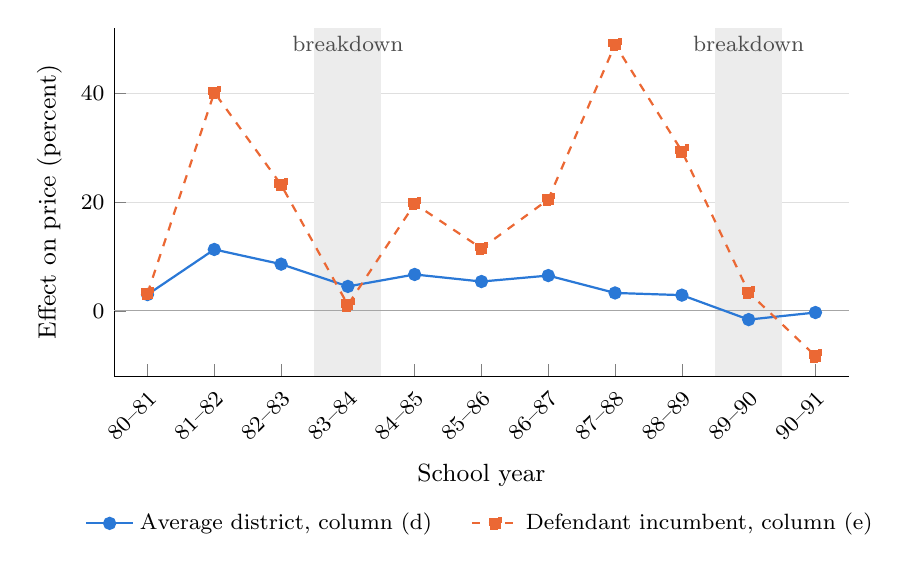
\begin{tikzpicture}
\begin{axis}[
  width=0.9\textwidth, height=6cm,
  xmin=0.5, xmax=11.5, ymin=-12, ymax=52,
  xtick={1,2,3,4,5,6,7,8,9,10,11},
  xticklabels={80--81,81--82,82--83,83--84,84--85,85--86,86--87,87--88,88--89,89--90,90--91},
  x tick label style={font=\footnotesize, rotate=45, anchor=north east},
  y tick label style={font=\footnotesize},
  xlabel={School year}, ylabel={Effect on price (percent)},
  label style={font=\small},
  legend style={font=\footnotesize, draw=none, fill=none, at={(0.5,-0.36)}, anchor=north, legend columns=2,
    /tikz/every even column/.append style={column sep=1.2em}}, legend cell align=left,
  axis lines*=left, ymajorgrids, grid style={gray!25}]
\fill[gray!15] (axis cs:3.5,-12) rectangle (axis cs:4.5,52);
\fill[gray!15] (axis cs:9.5,-12) rectangle (axis cs:10.5,52);
\draw[gray!70] (axis cs:0.5,0) -- (axis cs:11.5,0);
\addplot[thick, color={rgb,255:red,42;green,120;blue,214}, mark=*, mark size=2pt]
  coordinates {(1,3.0) (2,11.3) (3,8.6) (4,4.5) (5,6.7) (6,5.4) (7,6.5) (8,3.3) (9,2.9) (10,-1.6) (11,-0.3)};
\addlegendentry{Average district, column (d)}
\addplot[thick, dashed, color={rgb,255:red,235;green,104;blue,52}, mark=square*, mark size=2pt]
  coordinates {(1,3.2) (2,40.2) (3,23.2) (4,1.1) (5,19.7) (6,11.5) (7,20.5) (8,49.0) (9,29.4) (10,3.4) (11,-8.3)};
\addlegendentry{Defendant incumbent, column (e)}
\node[font=\footnotesize, gray!60!black, anchor=south] at (axis cs:4,46) {breakdown};
\node[font=\footnotesize, gray!60!black, anchor=south] at (axis cs:10,46) {breakdown};
\end{axis}
\end{tikzpicture}
\caption{Estimated effect of collusion on the price of school milk in southwestern Ohio, by school year. Shaded
years are the cartel breakdowns described in the testimony (1983--84 and 1989--90). Redrawn from
\citet{PorterZona1999}, Table~17, columns (d) and (e).}
\label{fig:13-pz99-effects}
\end{figure}

\begin{example}[From a log markup to damages]\label{ex:13-pz99-damages}
The dependent variable of \eqref{eq:13-pz99-damages} is the log price, so column (d) of \cref{tab:13-pz99-t17} is a
log difference, $\hat m = \ln p - \ln p^{\mathrm{bf}}$. The paper reports it as a percentage change (WP p.~31). As in
\eqref{eq:13-damages-log}, the overcharge as a share of spending is
\begin{equation*}
  \frac{p - p^{\mathrm{bf}}}{p} = 1 - e^{-\hat m} .
\end{equation*}
With $\hat m = 0.065$, the overcharge is $1 - e^{-0.065} = 6.3$ percent of spending. Reading 6.5 percent instead as a
ratio markup $\frac{p}{p^{\mathrm{bf}}} - 1$ would give $\frac{0.065}{1.065} = 6.1$ percent. A district that spent
\$100,000 on milk would have overpaid about \$6,300 (a hypothetical district, our computation). Because school milk demand is
nearly perfectly inelastic, this transfer is the whole of the district's loss.
\end{example}

The comparison with distance in the abstract can be checked against \cref{tab:13-pz99-control}. Fifty miles at the
base-model gradient of 0.0096 dollars per hundred miles adds 0.48 cents, or 3.6 percent of the mean price of 13.4
cents in \cref{tab:13-pz99-t1}. With bidder effects it adds 0.77 cents, or 5.7 percent (our computation). The authors'
own illustration is a district next to the plants of two conspirators whose nearest competitors are at least 50
miles away. Prices there could be about half a penny, or five percent, above the competitive level (WP p.~31).

\casehead{Critiques and limitations}
The evidence is a set of imperfect tests, none decisive alone. The likelihood ratio tests of equal slopes reject for
every defendant, and the authors note in footnote 15 that no single intercept represents all bidders. Such tests
would probably reject for many individual non-defendants too, so the rejections carry little weight by themselves.
The informative evidence is the pattern of deviations. Distance gradients are reversed and residuals are
correlated, and both match the testimony. Positive correlations could also arise from an omitted factor that affects
these firms alike (WP p.~27, footnote 28). The control group is assumed competitive. Collusion among non-defendants
would bias the benchmark toward the defendants' behavior and work against the tests.

The damage regression is a reduced form. Its identifying variation is the cross-sectional exposure of districts to
conspirators' plants, which is credible only if plant locations are unrelated to unobserved local cost and demand
conditions. The 75-mile radius, the plant-count shares and the quadratic forms are approximations, and the
competitive price for southwestern Ohio is predicted partly from districts elsewhere in the state. The year
pattern, which matches the breakdowns in the testimony, is the strongest validation of the index.

\casehead{Contribution}
The paper extends the Long Island design to markets in which collusion takes the form of incumbency rights and
territorial allocation. It models both the decision to bid and the level of the bid, with a selection correction. It
then matches several scheme-specific tests to the alleged scheme and builds a reduced-form damages estimate whose
time pattern can be compared with testimony. The combination of a competitive model estimated on a control group,
tests of independence across suspected firms, and damages from exposure to the ring remains a template for
procurement cases.

\casehead{Later screens}
Porter and Zona warn that a single test procedure able to detect all bid rigging is an impossible goal. Later work
has therefore developed tests aimed at particular schemes and data \citep[p.~210]{AskerNocke2021}.
\citet{BajariYe2003} test conditional independence and exchangeability (\cref{sec:13-detection-theory}).
\citet{AtheyLevinSeira2011} compare open and sealed timber auctions, as \cref{ch:auction-empirics} explains.
\citet{KawaiNakabayashi2020} exploit the rounds of Japanese national procurement auctions, as reported by
\citet[pp.~184--185]{AskerNocke2021}. When no first-round bid meets the secret reserve price, the lowest
first-round bid is announced and a second round follows. In the second round, the gap between the bids of the
first-round runner-up and the first-round winner is almost never negative. The gap between the bids of the
first-round third and second bidders often is. The first-round winner thus almost always wins again, while lower
ranks switch freely, which suggests that the winner was chosen before the auction. Applied across 2003--2006, the
test flags about 970 firms as collusive. \citet{ConleyDecarolis2016} detect groups of coordinating bidders in Italian
procurement, and \citet{OrtnerEtAl2020} develop screens that remain informative when cartels adapt to them.
\Cref{sec:12-eu-facts} uses the first two of these studies as evidence on the prevalence of collusion, and the book
does not develop the three tests further.

\section{Enforcement, Damages and What the Evidence Shows}\label{sec:13-enforcement}

The cartels of this chapter came to light in different ways, and the route matters for what they can teach. This
section describes the enforcement institutions and the selection of cartels they induce
(\cref{sec:13-institutions}). It then develops the methods used to measure the effects of collusion
(\cref{sec:13-damages}) and closes with what the evidence of the chapter shows (\cref{sec:13-synthesis}).

\subsection{Enforcement institutions and the selection of observed cartels}\label{sec:13-institutions}

\casehead{Law and penalties}
In the United States, Section~1 of the Sherman Act (1890) prohibits agreements in restraint of trade. Price fixing
is illegal per se \citep[p.~570]{Miller2010}. Section~1 is a criminal as well as a civil statute, so price fixing
and bid rigging can be prosecuted as crimes \citep[ch.~4, p.~74, footnote~13]{Kaplow2013}. Injured parties can sue for treble damages
\citep[p.~759]{Asker2010}.
In the European Union, Article~101 of the Treaty on the Functioning of the European Union prohibits cartels. The
European Commission imposes administrative fines, capped at 10 percent of a firm's turnover
\citep[p.~6]{ChenRey2013}. Page and footnote references to \citet{ChenRey2013} are to its working-paper version.
\Cref{tab:12-eu-fines} lists the largest fines the Commission has imposed. On the conventional view, liability for
price fixing requires proof of an agreement, usually through evidence of communication, and plus factors serve as
circumstantial support \citep[pp.~4, 21 and 109--110]{Kaplow2013}. \Cref{sec:12-kaplow} discusses Kaplow's critique of
this requirement, and \cref{sec:13-market-evidence} the market-based evidence itself.

\casehead{Leniency}
Proving an agreement is the hard part of enforcement, and leniency programs address it. The United States adopted a
corporate leniency program in 1978. Under the Antitrust Division's 1993 Corporate Leniency Policy, a firm that
reports before an investigation has begun receives leniency automatically if it meets six conditions. The Division
must have no information about the conduct from any other source. The firm must end its participation promptly,
cooperate fully and make restitution where possible, and its confession must be a corporate act rather than that of
individual executives. It must not have coerced others or led or originated the cartel. A firm
that misses these conditions, including one that comes forward after an investigation has begun, can still qualify
under seven alternative conditions. Four of them repeat the conditions on termination, cooperation, the corporate
confession and restitution. In addition, the firm must be the first to come forward and qualify. The Division must not yet
have evidence likely to yield a sustainable conviction, and it must judge that leniency would not be unfair to
others. \citet[p.~1]{ChenRey2013} summarize the revision as a first-informant rule and a post-investigation amnesty
rule. Eligibility after an investigation has begun thus depends on the alternative conditions.

The European Commission adopted its program in the 1996 Notice on the Non-Imposition or Reduction of Fines in
Cartel Cases. That notice reduced fines by 75 to 100 percent for a firm that reported before the Commission had
ordered an investigation. A firm that reported after such an investigation had failed to establish sufficient
grounds for proceedings could receive 50 to 75 percent. Both tiers also required the firm to be the first to adduce
decisive evidence, to end its involvement, to cooperate fully and not to have coerced others or instigated the
cartel. Other cooperation earned 10 to 50 percent. The first two
tiers are those that \citet[footnote~6]{ChenRey2013} describe. The Commission revised the program in 2002
\citep[footnote~1]{ChenRey2013} and again in its 2006 Notice on Immunity from Fines and Reduction of Fines in Cartel
Cases, which remains its framework. Under the 2006 notice, the first firm whose evidence enables an inspection or
a finding of infringement can obtain full immunity if it meets the notice's conditions. Later firms whose evidence
adds significant value receive reductions of 30 to 50 percent for the first, 20 to 30 percent for the second and up
to 20 percent for the others. Many recent prosecutions involve a whistleblower.

In the repeated-game language of \cref{ch:collusion-theory}, leniency changes both sides of a member's incentive
constraint. \citet[pp.~209--210]{AskerNocke2021} summarize the opposing effects identified by \citet{Harrington2008}.
The \emph{deviator amnesty effect} lets a member that undercuts its rivals also report the cartel and escape the
fine. Cheating becomes more attractive, which tightens the no-cheating constraint. The \emph{cartel amnesty effect}
works the other way. Lenient treatment of the first confessor lowers the expected fines that members pay, which
raises the value of colluding and eases the constraint. A third force, the \emph{race-to-the-courthouse effect},
counteracts the second (p.~209, note~77). A more lenient program can move the members from a state in which no
firm applies to one in which all race to report. Expected fines then rise and the value of colluding falls.
Leniency can also be exploited. If it is too generous, a cartel can collude and have members report in turn,
paying reduced fines. \citet{ChenRey2013} characterize the
optimal design. Some leniency before an investigation is always desirable. Leniency during an investigation is
desirable when investigations are unlikely to succeed without a report. Restricting leniency to the first informant
is useful, and their analysis does not support denying leniency to repeat offenders. The theory is developed in
\cref{ch:collusion-theory}.

Measuring the effect of a leniency program runs into the problem that cartels are unobserved
\citep[p.~209]{AskerNocke2021}. A rise in detected cartels after a program begins could reflect better detection or
more cartels. \citet{Miller2009} separates the two with a model of cartel formation, detection and dissolution. He
estimates it by Poisson regression on the U.S. indictments and information reports for violations of Section~1 from
1985 to 2005 \citep[pp.~186--187]{AskerNocke2021}. \Cref{rem:13-miller} shows the logic of his identification in
the notation of \cref{prop:13-selection}. The 1993 program raised cartel discoveries by about 60 percent, which
indicates better detection. Read through the model with the natural breakup rate held fixed, the later path of
discoveries indicates greater deterrence.

\casehead{How the cartels of this chapter came to light}
\Cref{tab:13-discovery} records the source of evidence for each case. The legal cartels left records because they
had no reason to hide. The prosecuted cases surfaced through complaints, wiretaps, convictions and confessions. Asker's
stamp ring collapsed after a dealer outside the ring alerted antitrust enforcement. Asker suggests that strong
members kept the weak ones partly because an expelled member could report the ring and seek leniency
(\cref{sec:13-asker}). A leniency program thus shapes the internal organization of a cartel as well as its
stability. \Cref{sec:13-market-evidence} classifies the kind of evidence that decided each case.

\begin{table}[htbp]
\centering
\caption{How the cartels studied in this chapter came to light}\label{tab:13-discovery}
\footnotesize
\begin{tabularx}{\textwidth}{@{}>{\raggedright\arraybackslash}p{4.1cm}>{\raggedright\arraybackslash}X@{}}
\toprule
Case & Source of evidence\\
\midrule
Joint Executive Committee, 1880--1886 & Open agreement before the Interstate Commerce Act, weekly cartel records and
trade-press reports of price wars\\
Sugar Institute, 1927--1936 & Trade association later ruled illegal by the Supreme Court, meeting notes kept by a
member\\
Bromine pools, 1885--1914 & Contracts, firm papers and trade press\\
Danish ready-mixed concrete, 1993--1996 & Prices published by the competition authority itself\\
Overlap group, 1950s--1991 & Department of Justice suit in 1991\\
Airline Tariff Publishing, 1990s & Department of Justice suit in 1992 and consent decrees\\
Quebec gasoline, 2002--2006 & Competition Bureau wiretaps, raids and guilty pleas\\
Lysine, citric acid and other industrial cartels, 1990s & Prosecutions and European Commission decisions\\
Stamp-auction ring, until 1997 & Complaint by a dealer outside the ring, faxed records kept by a member\\
Long Island paving, 1979--1985 & Federal conviction in 1984 and state and county suits\\
Ohio school milk, 1980--1990 & State suit, confessions by two dairies in 1993\\
\bottomrule
\end{tabularx}

\smallskip
\begin{minipage}{0.95\textwidth}\footnotesize
Notes: Compiled from the case studies of this chapter
(\cref{sec:13-jec,sec:13-legal,sec:13-information,sec:13-gasoline,sec:13-imperfect,sec:13-asker,sec:13-detection}).
\end{minipage}
\end{table}

\casehead{Selection}
We observe cartels that were legal or that were caught. Estimates of how long cartels last and how much they raise
prices are therefore conditional on detection. \citet{LevensteinSuslow2006} survey cross-section studies in which
average cartel duration ranges from 3.7 to 10 years (their Table~1). Their own sample covers 42 international
cartels prosecuted by the United States or the European Commission in the 1990s. These cartels lasted 5 years on
average, with a standard deviation of 4.5 and a range of 0 to 20 years (Table~1). Their text on p.~51 gives 5.4 years
and 4.7 for the same sample. The distribution of duration is bimodal. Many
cartels break up within a year, many last five to ten years, and some last decades (p.~43). They warn that ``in some
cases, samples are literally selected by prosecutors'' (p.~44). The surge in U.S. prosecutions of international
cartels followed the 1993 revision of the amnesty program (p.~50, footnote~21). Case-study samples
are selected differently, by researchers who choose industries with long or eventful cartel histories. Their mean
duration is 14 years, with a median of 6 (pp.~52--53).

Prosecuted cartels are also a small part of all cartels. The U.S.\ Department of Justice filed 92 criminal
cartel cases in 1982, with fines of \$36.8 million \citep[p.~182]{AskerNocke2021}. In 2017 it filed 21 cases, with
fines of \$2.79 billion. Fewer cases need not mean less collusion, because penalties, detection and the
size of the economy all changed. Where collusion can be measured directly, it is common.
\citet{KawaiNakabayashi2020} flag about 970 collusive firms in Japanese national procurement, and scaling up their
estimate implies that collusion affects about 0.85 percent of Japan's GDP. \citet[pp.~4, 6 and~29--30]{ConleyDecarolis2016}
estimate that groups of bidders whose entry and bids appear coordinated affected at least 30 percent of 802
average-bid roadwork auctions in northern Italy. Counties and municipalities in five regions held these auctions
between 2005 and 2010. When
Finnish cartels were legal and had to register, \citet{HyytinenSteenToivanen2018} count 900 of them between 1951
and 1990. \Cref{sec:12-eu-facts} discusses this evidence further.

Selection begins before detection, at formation. \citet[p.~187]{AskerNocke2021} write the participation
constraint of a potential member $i$ as
\begin{equation}\label{eq:13-participation}
  V_i^{\mathrm{comp}} \;\le\; V_i^{\mathrm{coll}} - \eta_i .
\end{equation}
Here $V_i^{\mathrm{coll}}$ is the firm's value inside the cartel, $V_i^{\mathrm{comp}}$ its value outside when the
other firms join, and $\eta_i$ a one-time cost of joining that captures the frictions of organizing. It is
constraint \eqref{eq:12-participation} of \cref{ch:collusion-theory}. A cartel forms only where the gain from collusion covers
these frictions for every member it needs. The cartels that exist are therefore already selected toward markets
with large collusive gains, before detection selects them again. The direction of the second bias depends on how
detection works, as a simple model shows.

\begin{proposition}[Duration of detected cartels]\label{prop:13-selection}
In each period of operation, a cartel breaks down for internal reasons with probability $q \in (0,1)$, so its
natural duration $L$ is geometric with $\E[L] = \frac{1}{q}$. Independently, in each period of operation it is
detected with probability $h \in (0,1)$. Let $r = (1-q)(1-h)$, a local symbol for the probability that a cartel
neither breaks down nor is detected in a period.
\begin{enumerate}[label=(\alph*)]
\item If detection uncovers the cartel without ending it, so that a cartel is eventually discovered if it is
detected in at least one period of its life, then
\begin{equation}\label{eq:13-sel-a}
  \E[L \mid \text{discovered}] = \frac{1-r}{h}\left[\frac{1}{q} - \frac{q(1-h)}{(1-r)^2}\right] > \frac{1}{q} .
\end{equation}
\item If detection ends the cartel, the observed duration of detected cartels satisfies
\begin{equation}\label{eq:13-sel-b}
  \E[L \mid \text{detected}] = \frac{1}{1-r} < \frac{1}{q} .
\end{equation}
\end{enumerate}
\end{proposition}

\begin{proof}
(a) A cartel of duration $L$ escapes detection with probability $(1-h)^L$, so the probability of discovery is
\begin{equation*}
  \Pr(\text{discovered}) = \sum_{L=1}^{\infty}q(1-q)^{L-1}\bigl[1 - (1-h)^L\bigr]
  = 1 - q(1-h)\sum_{L=1}^{\infty}r^{L-1} = 1 - \frac{q(1-h)}{1-r} = \frac{h}{1-r} ,
\end{equation*}
where the last step uses $1 - r - q(1-h) = 1 - (1-h)(1 - q + q) = h$. Using $\sum_{L\geq1}Lr^{L-1} = \frac{1}{(1-r)^2}$,
\begin{equation*}
  \E\bigl[L\,\indic\{\text{discovered}\}\bigr] = \frac{1}{q} - q(1-h)\sum_{L=1}^{\infty}L\,r^{L-1}
  = \frac{1}{q} - \frac{q(1-h)}{(1-r)^2} .
\end{equation*}
Dividing by $\Pr(\text{discovered})$ gives the equality in \eqref{eq:13-sel-a}. For the inequality, the
probability of discovery $1 - (1-h)^L$ is increasing in $L$. Two increasing functions of the same random variable
are positively correlated, so $\E[L\,(1-(1-h)^L)] > \E[L]\,\E[1-(1-h)^L]$, which is the inequality after division.

(b) A cartel survives each period with probability $r$, so it is detected in period $\ell$ with probability
$r^{\ell-1}h$. Conditional on detection, the duration is geometric with parameter $1-r$ and mean $\frac{1}{1-r}$.
Since $1 - r = q + h(1-q) > q$, this mean is below $\frac{1}{q}$.
\end{proof}

With $q = 0.2$, so that the natural mean duration is 5 years, and a detection probability of $h = 0.05$ per year,
cartels discovered after the fact last 8.17 years on average. Cartels ended by detection last 4.17 years. With
$h = 0.2$ the figures are 6.78 and 2.78 years (our computation, \texttt{pz\_checks.py}). Prosecuted samples mix both
mechanisms, so their bias can go either way. The same logic applies to overcharges. Cartels with large overcharges
may draw complaints from customers and be overrepresented, while sophisticated cartels may evade detection and be
underrepresented. Legal cartels avoid detection-driven selection but face another one, since we study those whose
records survived.

\begin{remark}[Reading cartel discoveries]\label{rem:13-miller}
The model of \cref{prop:13-selection} also explains how \citet{Miller2009} reads enforcement statistics. Consider a
population of industries of mass one. In each period a competitive industry forms a cartel with probability $\phi$
(a local symbol). A cartel is detected with probability $h$ and otherwise breaks down with probability $q$, so it
survives the period with probability $r = (1-q)(1-h)$. An industry whose cartel ends returns to competition. In a
steady state, the flow into collusion equals the flow out of it:
\begin{equation*}
  \phi\,(1 - \bar\pi) = (1 - r)\,\bar\pi , \qquad \text{so} \qquad \bar\pi = \frac{\phi}{\phi + 1 - r} ,
\end{equation*}
where $\bar\pi$ is the share of industries that collude. Discoveries per period are $h\bar\pi$. Substituting
$1 - r = q + h(1 - q)$ and differentiating,
\begin{equation*}
  h\bar\pi = \frac{h\phi}{\phi + q + h(1 - q)} , \qquad
  \frac{\partial\,(h\bar\pi)}{\partial h} = \frac{\phi\,(\phi + q)}{\bigl[\phi + q + h(1 - q)\bigr]^{2}} > 0 .
\end{equation*}
Two predictions follow, which are those of Miller's model as summarized by \citet[p.~186]{AskerNocke2021}. When a
policy raises $h$, the share $\bar\pi$ cannot change at once, so discoveries jump in proportion to the rise in $h$.
An immediate rise in discoveries therefore reveals better detection. In the new steady state, a higher $h$ with
unchanged $\phi$ and $q$ would keep discoveries above their old level. Discoveries also fall with the natural
breakup probability, since
\begin{equation*}
  \frac{\partial\,(h\bar\pi)}{\partial q} = -\frac{h\phi\,(1 - h)}{\bigl[\phi + q + h(1 - q)\bigr]^{2}} < 0 .
\end{equation*}
Holding $q$ fixed, a long-run level of discoveries below the old one therefore requires a fall in the formation
rate $\phi$, which is deterrence. Without that restriction a rise in $q$ can produce the same decline. With
$\phi = h = q = 0.1$, discoveries are $\frac{0.01}{0.29} = 0.0345$ per period. Raising $h$ to 0.2 and $q$ to 0.9
with $\phi$ unchanged lowers them to $\frac{0.02}{1.02} = 0.0196$. Reading the decline as deterrence thus requires
ruling out a rise in natural breakups and other changes in the transition rates. The discrete-time version and
its timing are our simplification of Miller's model.
\end{remark}

\subsection{Measuring the effects of collusion}\label{sec:13-damages}

\casehead{Overcharges and damages}
Let $p_t$ be the price paid in period $t$, $Q_t$ the quantity bought and $p^{\mathrm{bf}}_t$ the \emph{but-for
price}, the price that would have prevailed without the cartel. The \emph{overcharge} is $p_t - p^{\mathrm{bf}}_t$
per unit, and overcharge damages are
\begin{equation}\label{eq:13-damages}
  D = \sum_t \bigl(p_t - p^{\mathrm{bf}}_t\bigr)Q_t .
\end{equation}
Most methods estimate the log overcharge $\tau_t = \ln p_t - \ln p^{\mathrm{bf}}_t$. Since
$p^{\mathrm{bf}}_t = p_te^{-\tau_t}$, damages in terms of observed spending are
\begin{equation}\label{eq:13-damages-log}
  D = \sum_t \bigl(1 - e^{-\tau_t}\bigr)\,p_tQ_t .
\end{equation}
Buyers also lose the surplus on units they no longer buy. The change in consumer surplus is
\begin{equation*}
  \Delta CS = -\int_{p^{\mathrm{bf}}}^{p}Q(s)\,ds \approx -\bigl(p - p^{\mathrm{bf}}\bigr)\,\frac{Q + Q^{\mathrm{bf}}}{2}
  = -\bigl(p - p^{\mathrm{bf}}\bigr)Q - \frac{1}{2}\bigl(p - p^{\mathrm{bf}}\bigr)\bigl(Q^{\mathrm{bf}} - Q\bigr) ,
\end{equation*}
where the approximation is exact for linear demand. The first term is the overcharge, a transfer to the cartel. The
second is the additional loss of consumer surplus on the units no longer bought. It equals the deadweight loss only
if the but-for price equals marginal cost. With a constant marginal cost $mc$ below $p^{\mathrm{bf}}$, the lost units
also forgo the but-for margin, and the loss of total surplus adds $\bigl(p^{\mathrm{bf}} - mc\bigr)\bigl(Q^{\mathrm{bf}}
- Q\bigr)$ to the triangle. Take demand $Q = 10 - p$, $mc = 0$, $p^{\mathrm{bf}} = 2$ and $p = 4$. The triangle is 2,
and the loss of total surplus is $2 + 2 \times 2 = 6$. In procurement with inelastic demand, as on Long Island and in Ohio,
$Q^{\mathrm{bf}} = Q$ and the overcharge is the whole loss.

Direct purchasers who resell pass part of an overcharge on. If a cartel raises a downstream firm's unit cost by
$\Delta w$ and downstream pass-through is $\rho$ (\cref{ch:theory}), the downstream price rises by about
$\rho\,\Delta w$. To first order, direct purchasers then bear $(1-\rho)\Delta w$ per unit and their customers bear
$\rho\,\Delta w$, apart from volume effects.

\casehead{Umbrella damages and the loss of welfare}
Overcharge damages measure only part of the harm. \citet[pp.~210--212]{AskerNocke2021} separate the measures of a
cartel's impact in a static market with a competitive fringe (\cref{fig:13-cartel-impact}). In their figure the
members' aggregate marginal cost $MC_1$ slopes upward and meets demand at the competitive price. For simplicity we
draw $MC_1$ constant, so the competitive price equals $MC_1$. Fringe firms have higher costs and are inactive under
competition. When the cartel restricts output, the price rises and fringe firms produce until their marginal cost
reaches the cartel price. The overcharge is the price increase, $AG$ in the figure. Antitrust
damages are the overcharge times the cartel's sales, the rectangle $GAHF$, and courts treble this measure.
\emph{Umbrella damages} are the overcharge times the fringe's sales, the rectangle $HCEF$. Buyers pay them to firms
outside the cartel that raise prices under its umbrella. Buyers also lose the triangle $CDE$ on units they no longer
buy. The three areas together make up the loss of consumer surplus $GACD$. Antitrust damages thus exclude both
umbrella damages and the consumers' share of the deadweight loss (pp.~211--212).

Total surplus calls for different areas. The overcharge on the cartel's sales is a transfer. \emph{Productive
inefficiency} is the extra resource cost $BCEF$ of output produced by high-cost fringe firms instead of the cartel's
members. With constant $MC_1$, as in our drawing, part of the umbrella overcharge is dissipated in this way. With
an upward-sloping $MC_1$, as in their figure, the points $F$ and $E$ lie below the competitive price. The area
$BCEF$ is then no longer contained in the umbrella rectangle. The total welfare loss $BFDC$ is the sum of productive
inefficiency and the deadweight loss $CDE$. With the illustrative curves of the figure, damages are 10, umbrella
damages 6 and the deadweight loss 8, so consumers lose 24. Productive inefficiency is 4.5, fringe firms keep 1.5 of
the umbrella overcharge, and the total welfare loss is 12.5 (our computation). In this illustrative example of our
own, umbrella damages are 37.5 percent of all overcharge damages. \citet{Caoui2020} measures a different ratio in the
Texas school milk cartel of 1980--1992. Per contract, umbrella damages conditional on a non-cartel firm winning are
at least 35 percent of cartel damages conditional on the cartel winning. The lower bound comes from an efficient
cartel, which always sends its lowest-cost member to bid. With a randomly chosen cartel bidder the two can be equal
in size. Asker and Nocke summarize the result in terms of total cartel damages
(p.~212, note~82). The ratio compares two conditional means per contract, and it gives no aggregate share without
the probabilities of each winner.

\begin{figure}[htbp]
\centering
\begin{tikzpicture}[x=0.95cm,y=0.62cm,font=\small]
\fill[blue!12] (0,2) rectangle (2.5,6);
\fill[orange!30] (2.5,2) rectangle (4,6);
\fill[gray!30] (4,2) -- (4,6) -- (8,2) -- cycle;
\fill[pattern=north east lines, pattern color=black!70] (2.5,2) -- (2.5,4) -- (4,6) -- (4,2) -- cycle;
\draw[->] (0,0) -- (10.8,0) node[below] {$Q$};
\draw[->] (0,0) -- (0,10.8) node[left] {$p$};
\draw[thick] (0,10) -- (10,0) node[pos=0.12, right] {Demand};
\draw[thick] (0,2) -- (10.3,2) node[right] {$MC_{1}$};
\draw[thick, dashed] (2.5,4) -- (5.5,8) node[right] {$MC_{\mathrm{fringe}}$};
\draw[densely dotted] (0,6) -- (4,6);
\draw[densely dotted] (2.5,0) -- (2.5,2);
\draw[densely dotted] (4,0) -- (4,2);
\draw[densely dotted] (8,0) -- (8,2);
\node[left] at (0,6) {$A$};
\node[left] at (0,2) {$G$};
\node[above left] at (2.5,6) {$H$};
\node[above right] at (4,6) {$C$};
\node[left] at (2.5,4) {$B$};
\node[below left] at (2.5,2) {$F$};
\node[below right] at (4,2) {$E$};
\node[above right] at (8,2) {$D$};
\node[below] at (2.5,0) {$Q_{\mathrm{cartel}}$};
\node[below, align=center] at (4.6,-0.05) {$Q_{\mathrm{cartel}}$\\$+\,Q_{\mathrm{fringe}}$};
\node[below] at (8,0) {$Q_{\mathrm{comp}}$};
\node[font=\footnotesize] at (1.25,4) {damages};
\node[font=\footnotesize, align=left, anchor=west] at (6.0,6.1) {umbrella damages $HCEF$,\\ productive inefficiency\\ $BCEF$ (hatched)};
\draw[->, thin] (5.95,6.1) -- (3.7,4.9);
\node[font=\footnotesize] at (5.2,2.7) {$CDE$};
\end{tikzpicture}
\caption{Measures of a cartel's impact with a competitive fringe. In our drawing the cartel's members have constant
marginal cost $MC_1$, which is also the competitive price $G$. The cartel sells $Q_{\mathrm{cartel}}$ at the price $A$, and fringe
firms with marginal cost $MC_{\mathrm{fringe}}$ add $Q_{\mathrm{fringe}}$. The overcharge is $AG$. Antitrust damages
are the rectangle $GAHF$, umbrella damages the rectangle $HCEF$ and the deadweight loss the triangle $CDE$.
Productive inefficiency is the hatched area $BCEF$, and the total welfare loss is $BFDC$. We redraw the
decomposition in \citet{AskerNocke2021}, Figure~5, which has an upward-sloping $MC_1$. We take $MC_1$ constant and
use illustrative linear curves (demand $p = 10 - Q$, $MC_1 = 2$, cartel price 6). The point $H$ is our addition.}
\label{fig:13-cartel-impact}
\end{figure}

\casehead{Attributing harm when other distortions are present}
Markets with cartels often have other distortions, such as taxes or market power outside the cartel. Which part of
the total distortion should be attributed to collusion? The next example, from \citet[pp.~212--213]{AskerNocke2021},
shows that the answer depends on the thought experiment.

\begin{example}[A cartel and a tax]\label{ex:13-tax-cartel}
Firms sell a homogeneous good at constant marginal cost $c$ and face inverse demand $p = a - bq$, with $a > c$. A
unit tax $t < a - c$ is levied on sellers. Without a cartel the firms compete in prices, and with a cartel they
act as a monopolist (Example~2.1 of Asker and Nocke). Bertrand competition without the tax gives $p^{c} = c$. With
the tax, competition drives the price to cost including the tax, $p^{t} = c + t$. A monopolist without the tax
maximizes $(p - c)\frac{a - p}{b}$. Its first-order condition is $a - p - (p - c) = 0$, so
$p^{k} = \frac{a + c}{2}$. With the tax it maximizes $(p - c - t)\frac{a - p}{b}$, and the same steps give
$p^{t+k} = \frac{a + c + t}{2}$. The total distortion is
\begin{equation*}
  p^{t+k} - p^{c} = \frac{a - c + t}{2} .
\end{equation*}
Two decompositions add up to it. If the tax comes first, the tax adds $p^{t} - p^{c} = t$ and the cartel adds
\begin{equation*}
  p^{t+k} - p^{t} = \frac{a + c + t}{2} - (c + t) = \frac{a - c - t}{2} .
\end{equation*}
If the cartel comes first, the cartel adds $p^{k} - p^{c} = \frac{a - c}{2}$ and the tax adds
$p^{t+k} - p^{k} = \frac{t}{2}$. With $a = 10$, $c = 2$ and $t = 2$, the four prices are 2, 4, 6 and 7. The cartel's
effect is 3 in the first decomposition and 4 in the second (our numbers).
\end{example}

The first decomposition measures the \emph{marginal} impact of the cartel, holding the other distortion fixed. The
second measures its \emph{inframarginal} impact, its effect in a world without other distortions (p.~213). In an
antitrust case, the but-for world holds everything else constant, so the marginal measure is almost always the
right one for damages. Comparisons with a control market, and structural models that recover costs or values from
first-order conditions, naturally measure marginal impacts, because they take other distortions as given
(pp.~213--214). The choice matters for the academic question of how much of a market's distortion collusion
explains. For OPEC's productive inefficiency the two measures are close
\citep{AskerCollardWexlerDeLoecker2019}. For total welfare they differ greatly
\citep{AskerCollardWexlerDeLoecker2021}, because the deadweight loss is sensitive to the counterfactual quantities
\citep[p.~214]{AskerNocke2021}.

The central problem of measurement is the but-for price, which is never observed. Four families of methods
estimate it. \Cref{tab:13-damage-methods} summarizes them.

\casehead{Before, during and after}
The simplest method compares prices during the cartel with prices before or after it, controlling for cost and
demand shifters $x_t$:
\begin{equation}\label{eq:13-bda}
  \ln p_t = x_t\beta + \tau D_t + e_t ,
\end{equation}
where $D_t$ marks cartel periods. Ordinary least squares estimates $\tau$ consistently if $\E[e_t \mid x_t, D_t] = 0$.
The comparison of published Danish concrete prices with consumer prices (\cref{sec:13-concrete}) is of this type, with
an estimated effect of about $\ln 1.19 - \ln 1.019 = 0.155$. So are Levenstein's comparisons of cooperative and
noncooperative bromine prices (\cref{sec:13-bromine}) and the Sugar Institute margins before and after 1927
(\cref{sec:13-sugar-institute}). Porter's regime comparison for the JEC is a version in which $D_t$ is latent and
estimated (\cref{sec:13-jec}).

Three threats are common. Cartels may form when prices are falling, which makes the before period a poor benchmark
\citep[p.~45]{LevensteinSuslow2006}. Prices after a cartel may stay high, because coordination persists or because
firms under investigation want to limit their liability. \citet[pp.~80--81]{LevensteinSuslow2006} report a survey of
twenty-five price-fixing cases between 1973 and 1984 in which prices four years after indictment were about 7
percent higher. Finally, the dates of the cartel may be wrong.

The choice of controls $x_t$ raises a further problem \citep[pp.~215--220]{MarshallMarx2012}. A cartel can
influence variables that look exogenous. It may set inventories, capacity utilization and advertising
strategically, and input prices may reflect its bargaining power with suppliers. Exchange rates can serve as cover
if the cartel times its increases to coincide with currency movements. Such variables should not enter a
regression estimated over both periods, because their coefficients would mix competitive and collusive responses.
Marshall and Marx prefer to estimate a predictive model on the benchmark period alone. They choose its variables by
how well it predicts blocks of benchmark data withheld from estimation, and then use it to predict but-for prices
in the cartel period. The coefficients of such a model are weights for prediction, without a structural
interpretation (p.~220). A path of actual prices well outside the model's predictions is their first super-plus
factor (\cref{sec:13-market-evidence}).

\begin{remark}[Misdated cartel periods]\label{rem:13-misclassification}
Suppose the analyst uses an indicator $\tilde D_t$ in place of the true $D_t$, with no other regressors, and the
error in dating is unrelated to $e_t$. Then $\E[\ln p_t \mid \tilde D_t] = \text{const} + \tau\Pr(D_t = 1 \mid \tilde
D_t)$, so the regression slope converges to
\begin{equation*}
  \plim \hat\tau = \tau\bigl[\Pr(D_t = 1 \mid \tilde D_t = 1) - \Pr(D_t = 1 \mid \tilde D_t = 0)\bigr] ,
\end{equation*}
which is smaller than $\tau$ in absolute value whenever dating errors occur. In the JEC, trade-press reports of price
wars often lead the estimated regime series at the start of a war (\cref{sec:13-jec}). Such disagreements attenuate
regime effects estimated with the wrong series.
\end{remark}

\casehead{Yardsticks and difference in differences}
A \emph{yardstick} is a comparable market that the cartel did not affect. With markets $m$ and periods $t$,
\begin{equation}\label{eq:13-did}
  \ln p_{mt} = a_m + \lambda_t + \tau\,(C_m \times A_t) + x_{mt}\beta + e_{mt} ,
\end{equation}
where $C_m$ marks cartelized markets, $A_t$ marks cartel periods, $a_m$ are market effects and $\lambda_t$ are period
effects ($\lambda_t$ is a local symbol). Without covariates and with two markets and two periods,
\begin{align*}
  \tau &= \bigl\{\E[\ln p_{mt} \mid C=1, A=1] - \E[\ln p_{mt} \mid C=1, A=0]\bigr\}\\
       &\quad - \bigl\{\E[\ln p_{mt} \mid C=0, A=1] - \E[\ln p_{mt} \mid C=0, A=0]\bigr\},
\end{align*}
because the first difference removes $a_m$ and the second removes $\lambda_t$. The identifying assumption is
parallel trends. Without the cartel, prices in the two markets would have moved alike, conditional on $x_{mt}$
(\cref{app:econometrics}, \cref{ch:mergers}).

The chapter offers three applications. \citet{ErutkuHildebrand2010} estimate that Sherbrooke gasoline prices fell
1.75 cents per liter (standard error 0.80) relative to Montreal after the cartel investigation became public.
Relative to Quebec City they rose 0.26 (0.82) (\cref{tab:13-eh-t6}). The estimate depends on the choice of control.
\citet{Miller2010} finds that fares in markets affected by the Airline Tariff Publishing case fell \$13.57 relative
to control markets during the investigation. They rose \$12.71 after the settlement, leaving no significant net
change (\cref{tab:13-miller-t2}). \citet{CarltonBambergerEpstein1995} use a cross-sectional yardstick, comparing Overlap
schools with other private colleges conditional on observables. The Ivy-plus-MIT coefficient of $-\$322$ (standard
error 679) has a 95 percent interval of $[-\$1{,}653, \$1{,}008]$ (\cref{tab:13-cbe-t6}, our computation), so the
data cannot rule out sizable effects.

The main threats are contamination and differential shocks. Firms outside a cartel often raise their prices under
its umbrella. If the yardstick market is affected in this way, $\hat\tau$ is biased toward zero. With a single treated
market, inference relies on the time-series behavior of one pair of markets.

\casehead{Collusion-index regressions}
The regression \eqref{eq:13-pz99-damages} of \citet{PorterZona1999} replaces a binary treatment with a continuous
measure of exposure to the ring. The identifying variation is cross-sectional. Districts with more conspirators'
plants nearby should pay more, holding market structure and costs fixed. The assumption is that exposure is
unrelated to unobserved local price determinants. The year-by-year coefficients provide a check against the dates of
known breakdowns.

\casehead{Structural counterfactuals}
The most demanding method estimates the primitives of a model of collusive behavior and simulates the competitive
outcome. \citet{Asker2010} recovers the stamp dealers' value distributions from knockout bids and simulates
competitive target auctions (\cref{sec:13-asker}). True damages to sellers are \$36.99 or \$26.50 per ring win under
his two bounding assumptions, against naive damages of \$74.21 (\cref{tab:13-asker-t7}). The ratios are 0.50 and 0.36
(our computation). Naive damages overstate harm because knockout bids exceed values. \citet{ClarkHoude2013} simulate
incentive constraints and the value of delays as transfers (\cref{sec:13-clarkhoude}). Porter's reduced form for the
JEC predicts a price 66 percent higher in cooperative weeks (\cref{tab:13-porter-t4}). Structural estimates depend on
the assumed but-for conduct, for example Bertrand or Cournot, which the data may not pin down (\cref{ch:conduct},
\cref{prop:13-obs-equiv}).

\casehead{What collusion costs}
Estimates of the effects of collusion vary widely. \citet{ConnorBolotova2006} compile overcharges for 395 cartel
episodes from sources that reach back to 1770. The median overcharge is 19 percent and the mean 29 percent, with a
range from $-10$ to 322 percent \citep[pp.~214--215]{AskerNocke2021}. \Cref{tab:13-overcharge-surveys} adds the six
surveys collected by \citet[Table~7]{ErutkuHildebrand2010}. Their means range from 7.7 to 49 percent and their
medians from 7.8 to 44.5 percent. Against these numbers, the Sherbrooke overcharge of 2.7 percent is small and the
Ohio school milk estimate of about 6.5 percent is modest. Prices fell by at least 20 percent when the German cement
cartel of 1991--2002 collapsed \citep[p.~198]{AskerNocke2021}. Measured against the post-collapse price, the
overcharge was thus at least $\frac{0.2}{0.8} = 25$ percent (our computation). This lower bound lies between the
median and the mean of the Connor and Bolotova sample. Asker and Nocke describe it as a roughly 20 percent
overcharge, unremarkable compared with other cartels (p.~198, note~53).

\begin{table}[htbp]
\centering
\caption{Surveys of cartel overcharges}\label{tab:13-overcharge-surveys}
\small
\begin{tabular}{@{}lccc@{}}
\toprule
Survey & Cartels & Mean overcharge (\%) & Median overcharge (\%)\\
\midrule
Cohen and Scheffman (1989) & 5--7 & 7.7--10.8 & 7.8--14.0\\
Werden (2003) & 13 & 21 & 18\\
Posner (2001) & 12 & 49 & 38\\
Levenstein and Suslow (2002) & 22 & 43 & 44.5\\
Griffin (1989) & 38 & 46 & 44\\
OECD (2003) & 12 & 15.75 & 12.75\\
\addlinespace
\citet{ConnorBolotova2006} & 395 & 29 & 19\\
\bottomrule
\end{tabular}

\smallskip
\begin{minipage}{0.86\textwidth}\footnotesize
Notes: The first six rows reproduce \citet{ErutkuHildebrand2010}, Table~7, who take them from a compilation by
Connor. The surveys are named as in that table. The last row is from \citet[p.~215]{AskerNocke2021}.
\end{minipage}
\end{table}

Price effects alone say little about welfare. \citet{Barkley2020} studies a cartel of the four largest generic
insulin manufacturers in Mexico from 2003 to 2007, as reported by \citet[p.~215]{AskerNocke2021}. Bid rigging kept
prices stable until a large public health-care provider changed its procurement design, which destabilized the
cartel. Competitive bidding more than doubled the supply of insulin to the provider's patients. The number of
patients with access to insulin rose 42 percent, diabetes-related complications fell 25 percent and
diabetes-related deaths fell 3.4 percent. At the other end of the scale is OPEC.
\citet{AskerCollardWexlerDeLoecker2019} estimate total distortions in the allocation of world oil extraction of
\$744 billion in net present value. Of this, 14 to 22 percent is attributable to OPEC's market power
\citep[p.~214]{AskerNocke2021}.
Between 1970 and 2014, OPEC generated \$148 to \$233 billion of productive inefficiency and total welfare losses
between \$700 billion and \$5.7 trillion, in 2014 dollars \citep{AskerCollardWexlerDeLoecker2019,
AskerCollardWexlerDeLoecker2021}. The two OPEC figures for productive inefficiency are not directly comparable.
The 14 to 22 percent share of the \$744 billion net present value is \$104 to \$164 billion (our computation).
The \$148 to \$233 billion range is an inframarginal measure in 2014 dollars. Its width reflects different
assumptions about OPEC's effect on the internal efficiency of its members' production \citep[p.~215,
note~92]{AskerNocke2021}. The range for total welfare reflects the gap between the marginal and inframarginal
approaches (note~92). The largest estimate is about 0.15 percent of world GDP over the period
\citep[pp.~215--216]{AskerNocke2021}. Collusion of this scale can affect the aggregate economy.

\begin{table}[htbp]
\centering
\caption{Methods for measuring the effects of collusion}\label{tab:13-damage-methods}
\footnotesize
\begin{tabularx}{\textwidth}{@{}>{\raggedright\arraybackslash}p{2.3cm}>{\raggedright\arraybackslash}p{3.3cm}>{\raggedright\arraybackslash}X>{\raggedright\arraybackslash}X>{\raggedright\arraybackslash}p{2.6cm}@{}}
\toprule
Method & Estimating equation & Identifying assumption & Main threats & Examples\\
\midrule
Before, during and after & \eqref{eq:13-bda} & Cartel periods unrelated to unobserved cost and demand shocks & Cartels form
when prices fall, sticky post-cartel prices, misdated periods & Concrete, bromine, Sugar Institute, JEC\\
\addlinespace
Yardstick, difference in differences & \eqref{eq:13-did} & Parallel trends in a market the cartel did not affect &
Umbrella pricing in the control, differential shocks, one treated unit & Quebec gasoline, ATPCO, Overlap\\
\addlinespace
Collusion index & \eqref{eq:13-pz99-damages} & Exposure to the ring unrelated to local unobservables & Endogenous
plant locations, functional form & Ohio school milk\\
\addlinespace
Structural counterfactual & Model of collusive conduct and its primitives & Correct model, equilibrium and but-for
conduct & Misspecification, conduct not identified & Stamp ring, Quebec delays, JEC\\
\bottomrule
\end{tabularx}

\smallskip
\begin{minipage}{0.95\textwidth}\footnotesize
Notes: Our summary. Equation numbers refer to this chapter.
\end{minipage}
\end{table}

\subsection{What the evidence shows}\label{sec:13-synthesis}

\Cref{tab:13-synthesis,tab:13-synthesis-b} collect the cases of this chapter. For each case they report the setting,
the type of evidence, the data and method, the key quantitative finding and what it says about the theories of
\cref{ch:collusion-theory}.

\begin{table}[htbp]
\centering
\caption{What the evidence shows: legal cartels, information and gasoline}\label{tab:13-synthesis}
\scriptsize
\begin{tabularx}{\textwidth}{@{}>{\raggedright\arraybackslash}p{2.35cm}>{\raggedright\arraybackslash}p{1.7cm}>{\raggedright\arraybackslash}p{2.75cm}>{\raggedright\arraybackslash}X>{\raggedright\arraybackslash}p{3.0cm}@{}}
\toprule
Case & Evidence & Data and method & Key finding & Theory\\
\midrule
\citet{Porter1983}: JEC railroad cartel, 1880--1886 & Legal cartel & Weekly rates and tonnage, switching simultaneous
equations, EM & Price 66\% higher and quantity 33\% lower in cooperative weeks, conduct $\theta = 0.336$ (Tables
3--4) & Price wars on the equilibrium path \citep{GreenPorter1984}, prices below static monopoly\\
\addlinespace
\citet{Ellison1994}: JEC re-examined & Legal cartel & Markov switching with logit transitions, serially correlated
demand & Unanticipated demand innovations predict wars, coefficient $-4.15$ (2.64) (Table 3), weekly probability
0.975 that collusion continues, implied by Table 2 & Triggers of \citet{GreenPorter1984} fit better than booms
\citep{RotembergSaloner1986}, some secret cuts\\
\addlinespace
\citet{GenesoveMullin2001}: Sugar Institute, 1927--1936 & Legal trade association, narrative & Meeting notes, direct
marginal cost and Lerner index & Lerner index from 0.031 (1925--27) to 0.080 (1928--30) (Table 1) & Monitoring rules
\citep{Stigler1964}, limited retaliation against cheating\\
\addlinespace
\citet{Levenstein1997}: bromine, 1885--1914 & Legal pools, narrative & Trade press and firm papers, Markov tests of
war regimes & Shields pool price 40.88 vs 24.75 cents. After 1902, 29.3 vs 16.8 cents in cooperation and war & Short
wars from imperfect information, long wars from bargaining\\
\addlinespace
\citet{AlbaekMollgaardOvergaard1997}: Danish concrete, 1993--1995 & Government-assisted transparency & Published
transaction prices, before-after against price indices & Prices of reported grades up 19\% from January to October
1994, consumer prices up 1.9\% & Transparency facilitates collusion (\cref{prop:13-transparency})\\
\addlinespace
\citet{Miller2010}: Airline Tariff Publishing, 1991--1995 & Prosecuted facilitating practice & Ticket sample;
difference in differences, affected vs control routes & Relative fares $-\$13.57$ during the investigation,
$+\$12.71$ after settlement, no net change (Table 2) & Signaling, remedies that leave monitoring intact\\
\addlinespace
\citet{CarltonBambergerEpstein1995}: Overlap group, 1984--1990 & Prosecuted nonprofits & Cross-section of colleges;
regression with Overlap indicators & Ivy-plus-MIT effect $-\$322$ (679), insignificant (Table 6) & Agreement on aid
rules need not raise mean prices, low power\\
\addlinespace
\citet{BorensteinShepard1996}: 59 U.S.\ cities, 1986--1991 & Tacit, no case & Monthly margins, 2SLS on expected demand
and cost & Margin elasticities 0.37 to expected demand and $-0.37$ to expected cost (Table 2) & Collusive margins
follow expected future demand\\
\addlinespace
\citet{Noel2007}: Toronto, 2001 & Competitive benchmark & Twelve-hourly station prices, Markov switching & Asymmetric
cycles: relenting jumps of 5.6 cents per liter, cycle of 13.8 half-days (Tables II--III) & Competitive Edgeworth
cycles\\
\addlinespace
\citet{ClarkHoude2013}: Quebec, 2002--2006 & Prosecuted, wiretaps & Court documents, logit demand, simulated incentive
constraints & Timed delays raise low-cost firms' volumes 4--6\% (Table 7) & Transfers within a cartel
\citep{HarringtonSkrzypacz2011}\\
\addlinespace
\citet{ErutkuHildebrand2010}: Sherbrooke, 2005--2007 & Prosecuted, end of cartel & Weekly prices, difference in
differences & $-1.75$ (0.80) cents per liter vs Montreal, 0.26 (0.82) vs Quebec City (Table 6) & Overcharge
estimates depend on the control market\\
\bottomrule
\end{tabularx}

\smallskip
\begin{minipage}{0.95\textwidth}\footnotesize
Notes: Our summary of \cref{sec:13-jec,sec:13-legal,sec:13-information,sec:13-gasoline}. Table numbers refer to
the cited papers.
\end{minipage}
\end{table}

\begin{table}[htbp]
\centering
\caption{What the evidence shows: prosecuted cartels and statistical detection}\label{tab:13-synthesis-b}
\scriptsize
\begin{tabularx}{\textwidth}{@{}>{\raggedright\arraybackslash}p{2.35cm}>{\raggedright\arraybackslash}p{1.7cm}>{\raggedright\arraybackslash}p{2.75cm}>{\raggedright\arraybackslash}X>{\raggedright\arraybackslash}p{3.0cm}@{}}
\toprule
Case & Evidence & Data and method & Key finding & Theory\\
\midrule
\citet{BernheimMadsen2017}: lysine, nucleotides, citric acid, EC decisions 2000--2005 & Prosecuted & Case records &
9 of 22 Commission decisions describe discordant cartels, 6 fully concordant (footnote 2), deviations often
unpunished & Tolerated business stealing in imperfect cartels\\
\addlinespace
\citet{Asker2010}: New York stamp auctions, 1996--1997 & Prosecuted bidding ring & Knockout records, structural
private-values model & Seller damages \$36.99 or \$26.50 per ring win vs naive \$74.21 (Table 7) & Knockout design
induces overbidding, weak members subsidized\\
\addlinespace
\citet{PorterZona1993}: Long Island paving, 1979--1985 & Detection, with convictions & Public bids, GLS and
rank-ordered logit & Cartel ranks LR 8.94, $p = 0.06$, competitive ranks LR 4.3, $p = 0.64$ (Tables 5--6) &
Complementary bidding\\
\addlinespace
\citet{PorterZona1999}: Ohio school milk, 1980--1990 & Detection, with confessions & Bids, probit with selection
correction, residual correlations, collusion index & Average overcharge about 6.5\%, small in the breakdown
years, especially conditional on incumbency (Table 17) & Complementary bidding and territorial allocation, multimarket contact\\
\bottomrule
\end{tabularx}

\smallskip
\begin{minipage}{0.95\textwidth}\footnotesize
Notes: Our summary of \cref{sec:13-imperfect,sec:13-asker,sec:13-detection}. Table numbers refer to the cited
papers.
\end{minipage}
\end{table}

\casehead{Lessons}
Six lessons emerge.
\begin{enumerate}[label=(\arabic*)]
\item \emph{When collusion works, it raises prices substantially, and its effects vary widely.} Cooperative JEC
rates were 66 percent above war rates. Bromine pool prices were 65 to 75 percent above prices in noncooperative
periods. The Sugar Institute more than doubled the Lerner index, published concrete prices rose 15 to 20 percent
within a year, and Ohio school milk cost about 6.5 percent more. Across 395 episodes compiled by
\citet{ConnorBolotova2006}, the median overcharge is 19 percent and the mean 29 percent, with a range from $-10$ to
322 percent. Some cartels achieve much less. The Sherbrooke overcharge was 2.7 percent, and the Overlap estimate
cannot be distinguished from zero. Welfare losses can exceed what overcharges suggest. The collapse of a Mexican
insulin cartel cut diabetes-related deaths by 3.4 percent, and OPEC's welfare cost may reach trillions of dollars
(\cref{sec:13-damages}).
\item \emph{Price wars are real, but they have more than one cause.} The JEC wars fit the monitoring logic of
\citet{GreenPorter1984}, and Ellison's evidence favors triggers over booms. Levenstein's long bromine wars were
bargaining over the division of rents after entry or the expiry of contracts.
\item \emph{Statistical detection works when part of the market stays outside the ring.} The tests of \citet{PorterZona1993,PorterZona1999} use the firms outside
the ring to define competitive behavior. An inclusive ring can disguise itself. A
rejection of the competitive model for one group of firms is evidence that falls short of proof.
\item \emph{Internal organization matters.} Successful cartels relied on rules that close channels for secret price
cuts, on communication, on transfers through delays or inter-firm sales, and on knockout auctions. Cheating was
common and often tolerated, as \citet{BernheimMadsen2017} predict.
\item \emph{Price patterns alone rarely identify collusion.} Parallel prices are no evidence, and a price increase
becomes informative only together with quantities, costs and the allocation of output
(\cref{prop:13-kaplow-signs}). Asymmetric cycles appear in competitive Toronto and in the Quebec cartel. Margins
that track expected demand are evidence of tacit collusion only through a specific dynamic restriction. Plus
factors that are weak alone can be strong together (\cref{rem:13-plus-bayes}).
\item \emph{Credible inference needs a competitive benchmark and a theory of the specific scheme.} The most
convincing studies combine a model of competitive behavior, a restriction that a particular collusive scheme
violates, and outside information, such as testimony or wiretaps, that confirms the mechanism.
\end{enumerate}

\casehead{Connections}
Several threads continue elsewhere in the book. \Cref{ch:auction-empirics} develops the test of
\citet{AtheyLevinSeira2011} for collusion among mills in open timber auctions. Competitive and collusive behavior
predict the same entry and allocation there, and differ only in prices in sales with two or more mills. Northern
open-auction prices lie between the competitive and the fully collusive predictions.
\Cref{ch:mergers} discusses coordinated effects of mergers, which arise when a merger makes tacit collusion easier,
as in the analysis of the MillerCoors joint venture. \Cref{ch:discrete} presents the test of \citet{Bresnahan1987}
of collusion against competition in the 1955 automobile price war, which nests the two conduct hypotheses in one
model of demand and supply.
